\documentclass[aps,pre,twocolumn,superscriptaddress]{revtex4-2}

\usepackage[utf8]{inputenc}
\usepackage[T1]{fontenc}
\usepackage{graphicx}
\graphicspath{{../../figures/}}
\usepackage{amsmath,amsthm}
\usepackage{amssymb}
\usepackage{nicefrac}
\usepackage{tikz}
\usepackage{hyperref} % hyperref should be loaded late
\usepackage{cleveref}
\usepackage{subcaption}
\usepackage{orcidlink}
\usepackage{booktabs}

%\usetikzlibrary{positioning,arrows.meta,fit,calc}

\begin{document}

% --- Document Information ---
\title{
Simulation-Based Inference for Plant-Wide Fault Diagnosis and 
Artefactual Non-Identifiability Under
Closed-Loop Control
}

\author{Simone Casolo \orcidlink{0000-0003-2945-8931}
}
\email{simone.casolo@cognite.com} 
\affiliation{Cognite AS, Oslo, Norway}

\author{Alexander Johannes Stasik \orcidlink{0000-0003-1646-2472}}
%\email{alexander.stasik@sintef.no} 

\affiliation{Department of Data Science, Norwegian University of Life Sciences, \AA s, Norway}
\affiliation{Department for Mathematics and Cybernetics, SINTEF Digital, Oslo, Norway}


\author{Signe Riemer-Sørensen\orcidlink{0000-0002-5308-7651}
}
\affiliation{Department for Mathematics and Cybernetics, SINTEF Digital, Oslo, Norway}

\date{\today}


\begin{abstract}
Fault diagnosis in feedback-controlled chemical processes is fundamentally
limited by the controller's tendency to compensate for degradation,
suppressing the parametric signatures that estimation methods rely on. We apply simulation-based inference
(SBI) across two systems of increasing complexity: a
PI-controlled CSTR (two fault parameters) and the Luyben
reactor-column-recycle benchmark (five fault parameters, three PI loops,
liquid recycle). SBI approximates the Bayesian posterior over degradation parameters by a neural spline flow trained on summary statistics of fixed-length
observation windows.
%We apply simulation-based inference (SBI)---training a neural spline flow to approximate the Bayesian posterior over degradation parameters from summary statistics of fixed-length observation windows---across two systems of increasing complexity: a PI-controlled CSTR (two fault parameters) and the Luyben reactor-column-recycle benchmark (five fault parameters, three PI loops, liquid recycle). 
Identifiability is characterised via Fisher information
analysis, validated with simulation-based calibration, and benchmarked
against extended Kalman filter and Markov chain Monte Carlo baselines.
For the CSTR, a %250--500$\times$ 
Fisher-information deficit on the jacket-fouling parameter is shown to be method-independent and irreducible across four independent inference paradigms. 
For the recycle plant, decentralised control initially appeared
to produce three joint, two-parameter non-identifiabilities. We introduce a
raw-trajectory Fisher-information check by recomputing the
identifiability analysis on the raw, unaggregated trajectory of the same
already-observed channels in place of whole-window summary
statistics, and show all three non-identifiable scenarios are theoretically resolvable.
%For the recycle plant, decentralised control initially appeared to produce three joint, two-parameter non-identifiabilities. We introduce a raw-trajectory Fisher-information check---recomputing the identifiability analysis on the raw, unaggregated trajectory of the same already-observed channels in place of whole-window summary statistics---and show all three collapse under it.
%: not only does the
%apparent correlation vanish, but the Fisher information matrix's condition
%number improves by two to three orders of magnitude, 
%ruling out that the
%collapse is merely an artefact of comparing feature spaces of different
%dimension. 
%A control on an unrelated parameter pair confirms the
%representation does not manufacture spurious coupling indiscriminately, and
%a feature-level decomposition identifies the shared-actuator mechanism
%responsible, generalising the finding beyond the two systems studied. 
Thermal-fault masking by integral temperature control represents a genuine, representation-independent identifiability limitation. The origin is not a joint confound but a scalar reduction in information. Moreover, a confound's cost to fault classification, depends on whether the confused parameters share a fault-taxonomy unit, not their raw
Fisher-information magnitude. We show how two retracted confounds of comparable
magnitude leave one fault class undamaged while collapsing another to zero.
We show how SBI enables closed-loop, multi-unit fault diagnosis without baseline comparison. SBI relies only on a simulator and is applicable when no tractable likelihood exist. It captures the non-Gaussian posteriors induced by closed-loop feedback physics-ab-initio, it estimates joint
posterior for multi-unit root-cause attribution, it amortises to
real-time inference, and it requires no historical labelled-fault data. 
%We recommend that any joint non-identifiability surfaced by a
%compressed-feature representation in closed-loop SBI be checked against the
%RT-FIM protocol before being reported as physical.
\end{abstract}

\maketitle

\noindent\textbf{Keywords:} condition monitoring, Bayesian statistics, 
simulation based inference, predictive maintenance, closed-loop identifiability, recycle process, 
prognostics and health management, fault diagnosis.

\section{Introduction}
\label{sec:related_work}

Continuous chemical processes such as reactor-separator-recycle configurations
are subject to progressive degradation: catalyst activity decays through
poisoning or sintering, heat-exchanger surfaces accumulate fouling deposits,
and separator efficiency erodes over operating cycles.  
Timely quantification
of such degradation is essential for risk-informed maintenance scheduling,
product quality assurance, and avoidance of unplanned shutdowns~\citep{Frank1990,Isermann2006}.
Current industrial practice relies on three broad families of tools~\citep{ZHAO2026112159, Huo2026}:
(i)~model-based observers, principally the extended and unscented Kalman filters
(EKF/UKF), which propagate Gaussian approximations of the joint state-and-parameter
posterior~\citep{Jazwinski1970,JulierUhlmann2004};
(ii)~multivariate statistical methods based on principal component analysis or
partial least squares, which provide sensitivity indices and alarms but not
calibrated parameter posteriors~\citep{Qin2012, Kini2024, Lou2021, Huo2026}; and
(iii)~data-driven anomaly detectors built on neural or recurrent architectures,
which flag deviations from normal operation without quantifying fault severity in
physically interpretable units~\citep{WU2018185, Jia2025, Feng2026, HAN2020161, HAN20258859}.
None of these approaches delivers a calibrated
probability distribution over the fault-parameter space needed for maintenance planning. The decision to schedule an
intervention depends on the probability that a parameter has crossed a critical
threshold, not on whether a point estimate has done so.

This diagnostic task is made structurally harder by the feedback controllers
that regulate the plant. Decentralised proportional-integral (PI) loops
compensate for degradation.
%: a fouled heat exchanger is countered by increasing
%the coolant flow; a deactivating catalyst is compensated by adjusting the
%temperature setpoint.  
It is a well-understood limitation that the control compensation suppresses the same parametric
signatures that estimation methods rely on \citep{Gustavsson1977, Forssell1999}. Critically, this method-independent limitation is rooted in the information content of the closed-loop data, and it affects Bayesian and frequentist, online and offline, neural and classical methods equally (see~\citealt{Ljung1999}, Ch.~13). A fixed operating setpoint with a high-gain
controller implies near-zero spectral excitation of the controlled variable in the frequency band where fault-parameter information is concentrated, driving the local Fisher information for thermally-masked parameters toward zero. The practical consequence for fault diagnosis is twofold: some parameters are fundamentally harder to estimate than others under closed-loop operation, and apparent joint non-identifiabilities that emerge in compressed feature representations may be artefacts of lossy temporal aggregation rather than properties of the plant.  Characterising and distinguishing these two effects (scalar information reduction versus representation artefact) is the central methodological problem this work addresses.

Simulation-based inference (SBI)~\citep{Cranmer2020} offers a route to full posterior inference that circumvents the two principal limitations of the existing baselines. By training a neural density estimator on simulated (parameter, observation) pairs rather than an explicit likelihood, SBI produces a fully amortised posterior approximation~\citep{Greenberg2019} that can be evaluated on any new observation window in a single forward pass. Three properties make this attractive for plant-wide condition monitoring:
\emph{(a) Amortisation} --- one offline training run of a few minutes yields
inference latency.
\emph{(b) Full non-Gaussian posteriors} --- the neural spline flow
architecture can represent multi-modal and banana-shaped
posterior geometry that the Gaussian approximation underlying Kalman filters cannot~\citep{Durkan2019}.
\emph{(c) No likelihood derivation} --- a process simulator is used directly without linearisation or closed-form noise-distribution assumptions.
Sequential Markov chain Monte Carlo provides equally full posteriors but carries a per-window inference cost for full plant systems, making it infeasible at the scale and cadence required.

This study contributes five results connected to SBI as a method for industrial fault detection. First, we characterise the closed-loop identifiability limitation for a PI-controlled CSTR: the Fisher information ratio is derived analytically and shown to be \emph{method-independent} by four fundamentally
different inference paradigms all recovering the same
bias. It is separately shown to be \emph{irreducible}.
Second, a trained neural spline flow achieves macro-F1~$= 0.990$ on six closed-loop fault scenarios at 16~ms per window, and tracks 30-day catalyst and fouling degradation within a few percent of the true value, with negligible bias.
%$\mathrm{MAE}_\alpha = 0.004$ and $\mathrm{MAE}_\beta = 0.033$.
Third, we investigate the Wu et al.~\citeyearpar{Wu2003} reactor-column-recycle benchmark
(Fig.~\ref{fig:system_schematic} consisting of five fault parameters, 14 scenarios, three PI loops),
considered a prototypical multi-unit plant-wide system with complex control
dynamics (snowball effect, actuator saturation, and nonlinear interactions).
Unit-level fault classification reaches 87.4\% accuracy (macro-F1~$=0.694$),
with near-perfect detection of reactor ($F_1=0.948$) and column ($F_1=1.000$)
faults. The lower macro-F1 is strongly driven by a single class whose
failure is explained by our fourth contribution below, not by a
general weakness of the plant-wide extension. Extended Kalman filters (EKF) 
achieves only a 3\% empirical coverage under snowball conditions, where SBI degrades gracefully.
Fourth, a Fisher-information diagnostic collapses three apparent joint parameter degeneracies in the recycle plant, showing them
to be artefacts of the observation representation rather than physical
properties of the plant, and reveals that a confound's consequence for fault
classification depends on whether the confused parameters share a
fault-taxonomy unit, not on the raw strength of the confound. Two artefacts
of comparable Fisher-information magnitude leave one fault class undamaged
($F_1=0.948$) while collapsing another to $F_1=0.000$. 
Fifth, we show that amortised SBI is structurally suited to closed-loop, multi-unit fault diagnosis without baseline comparison. It
requires only a stochastic simulator even where no tractable likelihood exists, it
captures the non-Gaussian posterior induced by closed-loop feedback physics, it estimates the joint posterior for multi-unit root-cause attribution, it amortises
to sub-20~ms inference aligned with continuos monitoring cadence, and requires no historical labelled-fault data.

\begin{figure*}[t]
    \centering
    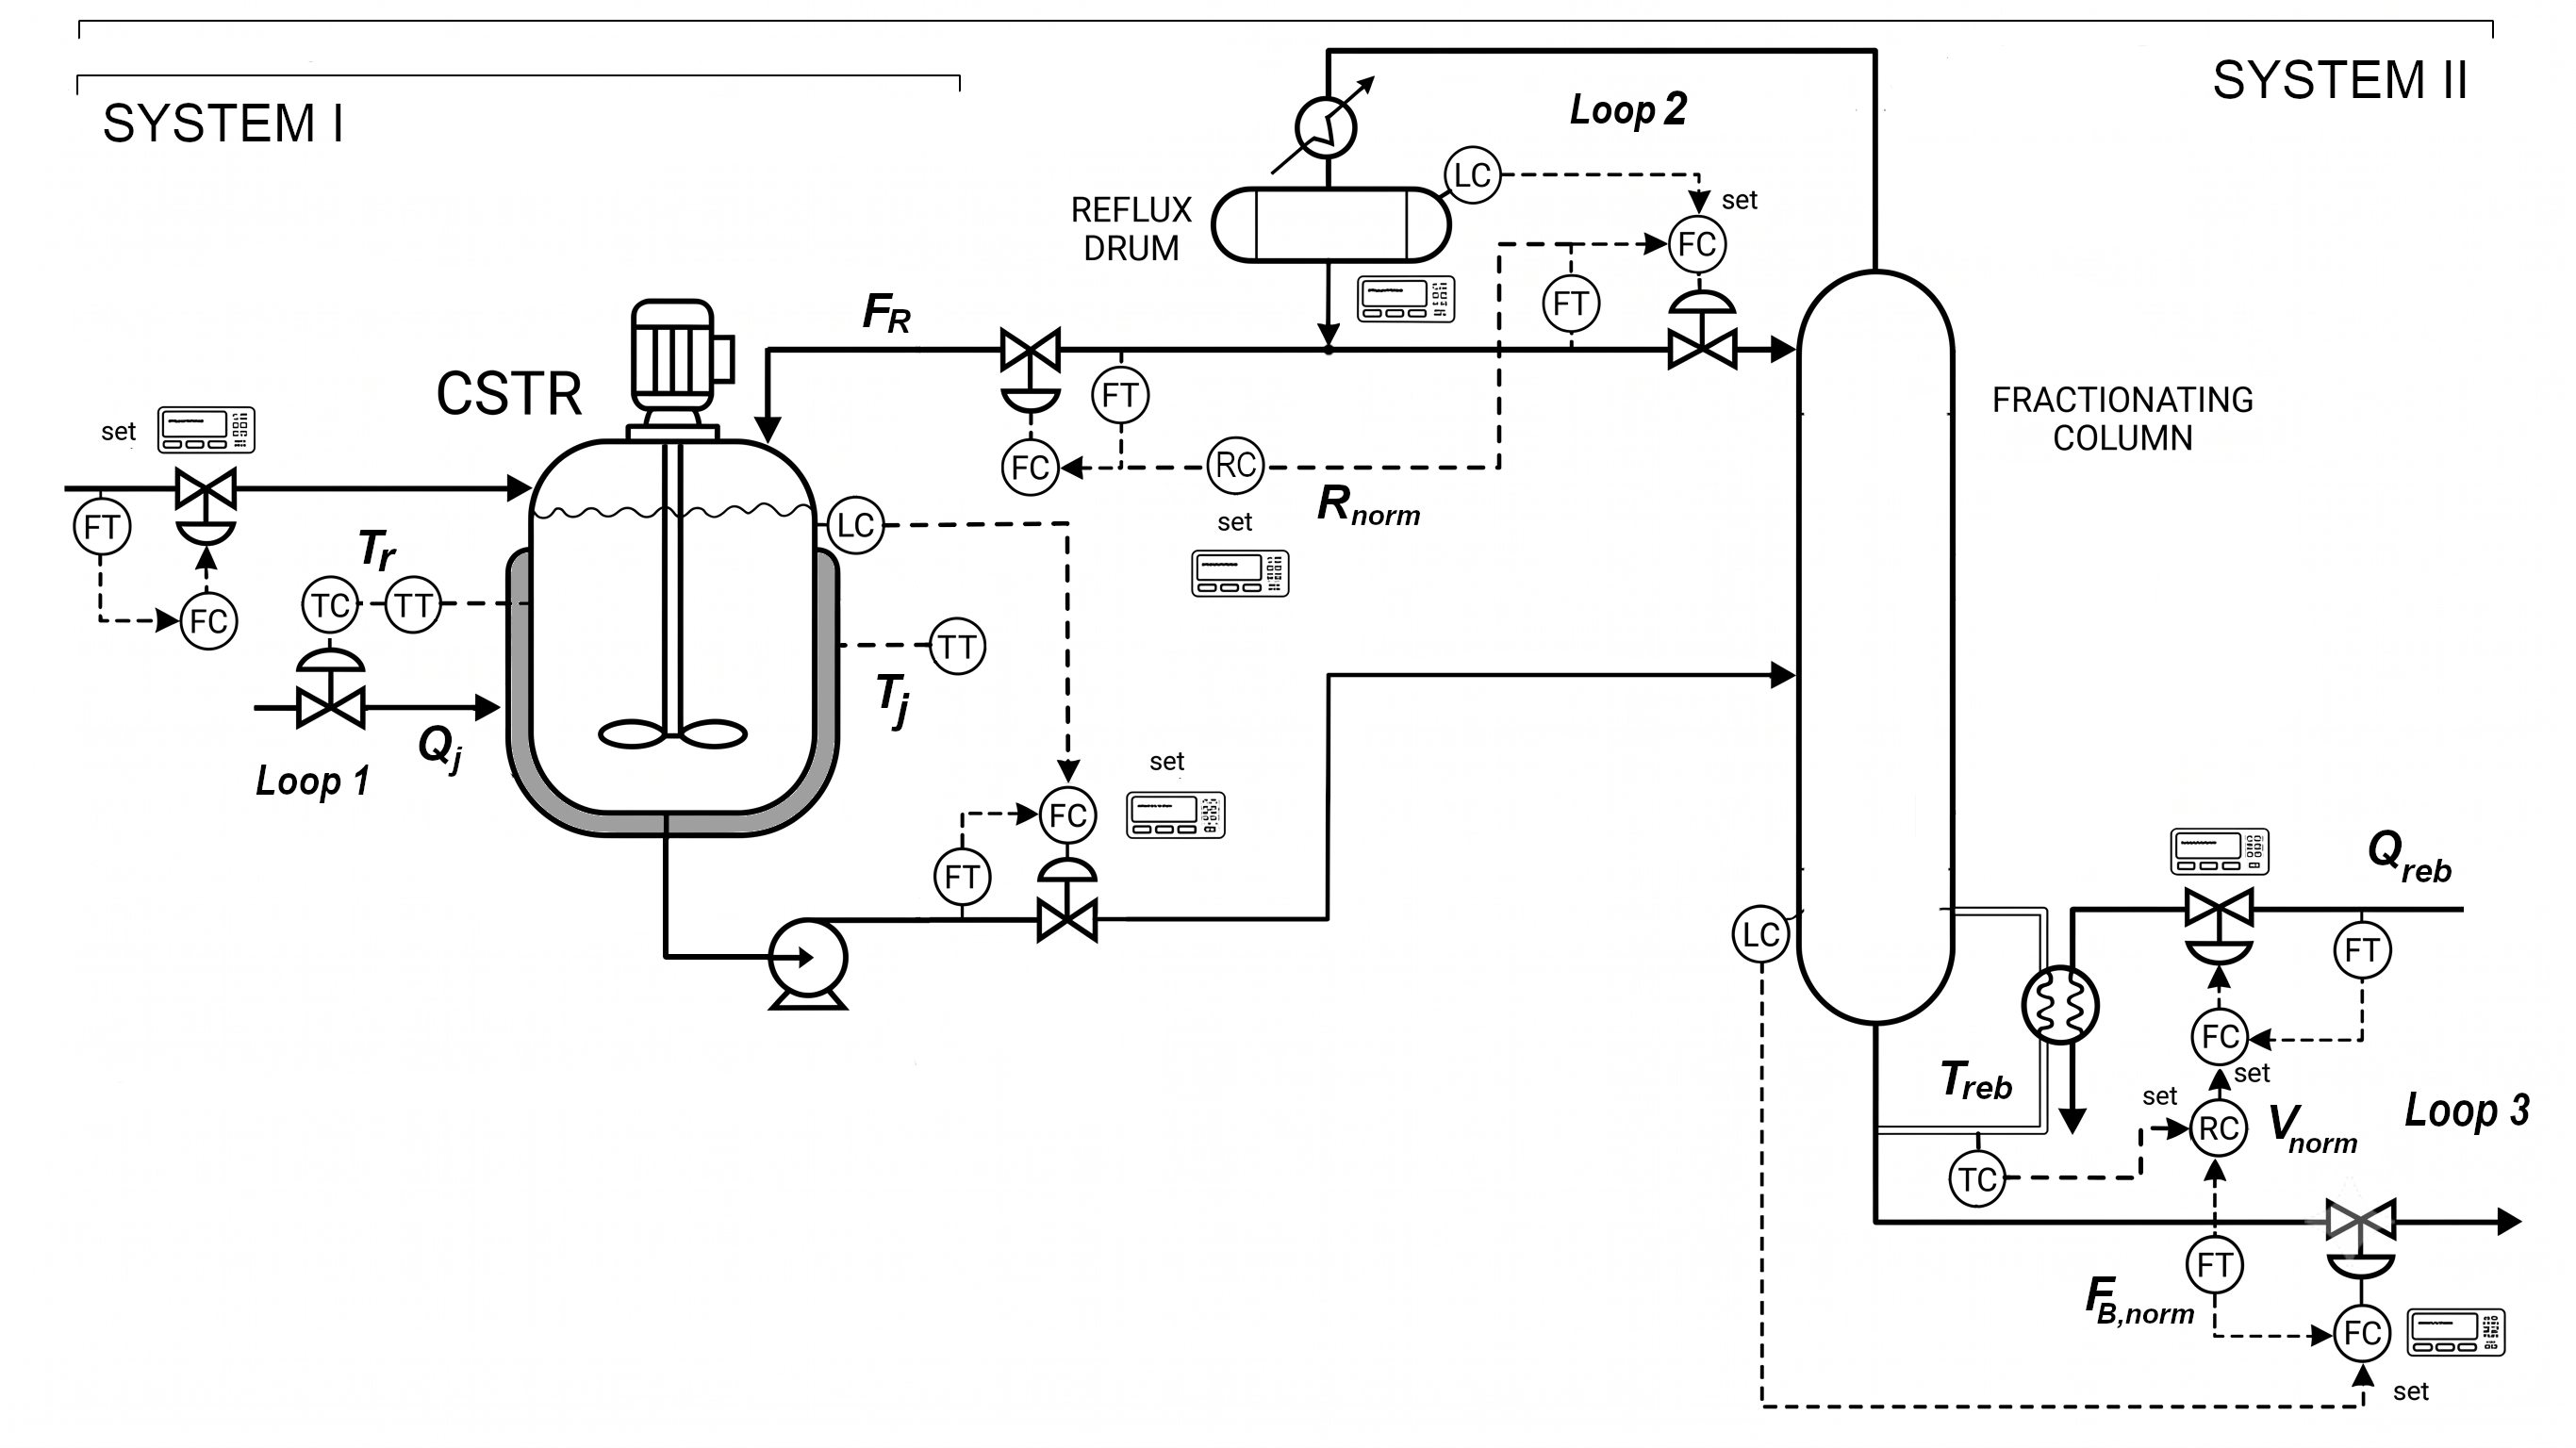
\includegraphics[width=0.9\linewidth]{PFD_Wu2003.png}
    \caption{Schematic of the two process systems studied.  System~I (left) 
     is a single propylene oxide CSTR under PI temperature
      control.  System~II (full diagram) is the Luyben reactor-column-recycle
      benchmark~\citep{Wu2003} consisting of a CSTR coupled to a distillation column
      with liquid recycle and three decentralized PI loops.}
    \label{fig:system_schematic}
\end{figure*}

\section {System~I: CSTR with PI Temperature Control}
\label{sec:system1}

Two systems of increasing complexity are studied. As shown in Figure \ref{fig:system_schematic}, System~I can be considered a sub-system of System~II, where System~I is a
single CSTR under proportional-integral temperature control, drawn from the canonical nonlinear CSTR benchmark of
Fogler~\citep{Fogler2016}. 
% with parameters representing propylene oxide hydrolysis reaction. 
%System~II is the Luyben
%reactor-column-recycle benchmark of~\citet{Wu2003} and depicted in 
%Fig.~\ref{fig:system_schematic}: a CSTR coupled to a distillation 
%column with liquid recycle and three decentralized PI loops.
%This section develops the full mathematical
%formulation for the two systems, motivates both the open- and closed-loop
%representations, and defines the fault parameterisation used throughout
%the study.
Specifically, we consider acid-catalysed liquid-phase hydrolysis of
propylene oxide (PO) to propylene glycol.
The reaction is pseudo-first-order in PO concentration, irreversible,
and mildly exothermic following an Arrhenius rate law.
Kinetic parameters are taken from Fogler
(2016), Module~13~\citep{Fogler2016}, whose values are traceable to the
original experimental measurements of \citet{Furusawa1969} for the
ring-opening of propylene oxide in dilute aqueous acid solution. 
%
%with pre-exponential factor $k_0 = 1.696\times10^{13}$~min$^{-1}$,
%activation energy $E_a = 75{,}362$~J~mol$^{-1}$, and universal gas
%constant $R = 8.314$~J~(mol~K)$^{-1}$.  

\subsection{Open-Loop Model}
\label{sec:open_loop}

In the absence of feedback control, the reactor is characterised by
three state variables: reactant concentration $C$~[mol~L$^{-1}$],
reactor temperature $T$~[K], and jacket temperature $T_c$~[K].  With
coolant flow rate $Q_c$ treated as a fixed external input, the
energy-balanced material model is
%
\begin{subequations}
\label{eq:open_loop}
\begin{align}
  \frac{dC}{dt}
    &= \frac{Q}{V}\bigl(C_i - C\bigr)
       - k(T)\,C,
  \label{eq:dC_ol} \\[4pt]
  \frac{dT}{dt}
    &= \frac{Q}{V}\bigl(T_i - T\bigr)
       - \frac{\Delta H_r}{\rho C_p}\,k(T)\,C
       - \frac{U\!A}{\rho C_p V}\bigl(T - T_c\bigr),
  \label{eq:dT_ol} \\[4pt]
  \frac{dT_c}{dt}
    &= \frac{Q_c}{V_c}\bigl(T_{ci} - T_c\bigr)
       + \frac{U\!A}{\rho_c C_{pc} V_c}\bigl(T - T_c\bigr).
  \label{eq:dTc_ol}
\end{align}
\end{subequations}
%

The standard enthalpy of reaction is negative $\Delta H_r = -84{,}666$~J~mol$^{-1}$ ($-20{,}220$~cal~mol$^{-1}$)~\citep{Fogler2016,Ziyai2022},
consistent with the ring-strain release enthalpy for the epoxide opening in aqueous solution~\citep{NIST_WebBook}. As $\Delta H_r < 0$, the term $-\Delta H_r / (\rho C_p)$ in Eq.~\eqref{eq:dT_ol} is positive, reflecting the exothermic heat release. The overall heat transfer coefficient-area product $U\!A$ [cal~min$^{-1}$~K$^{-1}$] couples the reactor and jacket energy balances. All nominal parameter values are listed in Table~\ref{tab:params_system1}.

The open-loop steady state is found by setting all time derivatives to zero and solving the resulting nonlinear algebraic system.  At the
nominal operating conditions (Table~\ref{tab:params_system1}) and $Q_c = Q_{c0} = 80$~L~min$^{-1}$, the system has a unique physically
meaningful steady state at
$C_\mathrm{ss} \approx 0.018$~mol~L$^{-1}$,
$T_\mathrm{ss} \approx 312.5$~K,
$T_{c,\mathrm{ss}} \approx 299.1$~K,
corresponding to a single-pass conversion of approximately 98\%. The open-loop model captures the essential coupling between reactor exothermicity and jacket cooling, and serves as the reference for understanding how feedback control modifies the observable system behaviour.




% ------------------------------------------------------------------
\begin{table*}[t]
\centering
\caption{Nominal parameter values for System~I (propylene oxide
  CSTR). Kinetic parameters from \citet{Fogler2016}
  (Module~13) based on \citet{Furusawa1969}, physical properties from
  \citet{PerrysHandbook}, controller tuning from the present work.}
\label{tab:params_system1}
\small
\begin{tabular}{lllll}
\toprule
Parameter & Symbol & Value & Units & Source \\
\hline
\midrule
\multicolumn{5}{l}{\textit{Reaction kinetics}} \\
Pre-exponential factor     & $k_0$          & $1.696\times10^{13}$ & min$^{-1}$            & \citet{Fogler2016} \\
Activation energy          & $E_a$          & 75{,}362             & J~mol$^{-1}$          & \citet{Fogler2016} \\
Standard heat of reaction  & $\Delta H_r$   & $-84{,}666$          & J~mol$^{-1}$          & \citet{Fogler2016,Ziyai2022} \\
Universal gas constant     & $R$            & 8.314                & J~(mol~K)$^{-1}$      & — \\
\midrule
\multicolumn{5}{l}{\textit{Reactor geometry and feed conditions}} \\
Reactor volume             & $V$            & 500                  & L                     & This work \\
Jacket volume              & $V_c$          & 40                   & L                     & This work \\
Volumetric feed flow       & $Q$            & 40                   & L~min$^{-1}$          & This work \\
Residence time             & $\tau = V/Q$   & 12.5                 & min                   & Derived \\
Inlet PO concentration     & $C_i$          & 0.97                 & mol~L$^{-1}$          & This work \\
Feed temperature           & $T_i$          & 297                  & K                     & This work \\
Coolant inlet temperature  & $T_{ci}$       & 297                  & K                     & This work \\
\midrule
\multicolumn{5}{l}{\textit{Physical properties}} \\
Reactor fluid density      & $\rho$         & 1{,}000              & g~L$^{-1}$            & \citet{PerrysHandbook} \\
Reactor fluid heat capacity & $C_p$         & 1.0                  & cal~(g~K)$^{-1}$      & \citet{PerrysHandbook} \\
Coolant density            & $\rho_c$       & 1{,}000              & g~L$^{-1}$            & \citet{PerrysHandbook} \\
Coolant heat capacity      & $C_{pc}$       & 1.0                  & cal~(g~K)$^{-1}$      & \citet{PerrysHandbook} \\
Heat transfer coefficient-area & $U\!A$     & 12{,}500             & cal~(min~K)$^{-1}$    & This work \\
\midrule
\multicolumn{5}{l}{\textit{PI controller}} \\
Temperature setpoint       & $T_\mathrm{sp}$ & 312.5               & K                     & This work \\
Proportional gain          & $K_p$          & 150                  & (L~min$^{-1}$)~K$^{-1}$ & This work \\
Integral time constant     & $\tau_i$       & 10                   & min                   & This work \\
Coolant flow bias          & $Q_{c0}$       & 80                   & L~min$^{-1}$          & This work \\
Coolant flow minimum       & $Q_{c,\min}$   & 0                    & L~min$^{-1}$          & Physical \\
Coolant flow maximum       & $Q_{c,\max}$   & 400                  & L~min$^{-1}$          & Physical \\
\midrule
\multicolumn{5}{l}{\textit{Fault parameter priors}} \\
Catalyst activity          & $\alpha$       & $\mathcal{U}(0.4,\,1.2)$ & — & This work \\
Jacket conductance         & $\beta$        & $\mathcal{U}(0.4,\,1.2)$ & — & This work \\
\hline
\bottomrule
\end{tabular}
\end{table*}
% ------------------------------------------------------------------

\subsection{Closed-Loop Model}
\label{sec:closed_loop}
%In industrial practice, continuous stirred-tank reactors operating at
%exothermic conditions are invariably equipped with feedback temperature
%controllers to prevent runaway and to maintain product quality.  
The closed-loop model employed in this work augments the open-loop
system in Eq.\eqref{eq:open_loop} with a proportional-integral (PI)
controller that manipulates the coolant flow rate $Q_c$ to regulate
reactor temperature at a setpoint $T_\mathrm{sp}$. In addition, the anti-windup integrator $I$
[K~min] accumulates the temperature error whenever the actuator is not saturated:

%\paragraph{State equations.}
%\begin{subequations} \label{eq:dI_cl}
\begin{equation}    
\label{eq:closed_loop}
 % \frac{dC}{dt}
 %   &= \frac{Q}{V}\bigl(C_i - C\bigr)
 %      - k(T)\,C,
%  \label{eq:dC_cl} \\[4pt]
 % \frac{dT}{dt}
 %   &= \frac{Q}{V}\bigl(T_i - T\bigr)
 %      - \frac{\Delta H_r}{\rho C_p}\,k(T)\,C
%       - \frac{U\!A}{\rho C_p V}\bigl(T - T_c\bigr),
 % \label{eq:dT_cl} \\[4pt]
%  \frac{dT_c}{dt}
%    &= \frac{Q_c}{V_c}\bigl(T_{ci} - T_c\bigr)
       %+ \frac{U\!A}{\rho_c C_{pc} V_c}\bigl(T - T_c\bigr),
       %\label{eq:dTc_cl} \\[4pt]
  \frac{dI}{dt} = \bigl(T - T_\mathrm{sp}\bigr)\cdot
       \mathbf{1}\!\left\{Q_{c,\min} < Q_c < Q_{c,\max}\right\},
%\end{align}
%\end{subequations}
\end{equation}
providing conditional anti-windup. The integrator accumulation is suspended whenever
the coolant valve is fully closed or fully open thereby preventing integrator
windup during periods of actuator saturation~\citep{Seborg2011}.

%\paragraph{PI control law.}
The coolant flow rate $Q_c$ [L~min$^{-1}$] is computed from the
parallel-form PI expression with actuator limits:
%
\begin{equation}
  Q_c = \mathrm{clip}\!\left(
    Q_{c0} + K_p\bigl(T - T_\mathrm{sp}\bigr) + \frac{I}{\tau_i},\;
    Q_{c,\min},\;
    Q_{c,\max}
  \right),
  \label{eq:pi_law}
\end{equation}
%
where $K_p = 150$~(L~min$^{-1}$)~K$^{-1}$ is the proportional gain,
$\tau_i = 10$~min is the integral time constant, $Q_{c0} = 80$~L~min$^{-1}$
is the bias (the nominal coolant flow at zero error), and
$[Q_{c,\min}, Q_{c,\max}] = [0, 400]$~L~min$^{-1}$ defines the physical
actuator range.  A positive gain is used throughout since an increase in
temperature above setpoint demands an increase in coolant flow
(direct-acting on the energy balance).
Under non-saturating, steady-state PI control
(i.e.\ $Q_{c,\min} < Q_c < Q_{c,\max}$, $dI/dt = 0$), integral action
drives the offset to zero and consequently, the closed-loop steady state satisfies
$T_\mathrm{ss} = T_\mathrm{sp}$ exactly, independently of the values of
the fault parameters.
% $\alpha$ and $\beta$ introduced in
%Section~\ref{sec:fault_params} below.  
This is the fundamental closed-loop masking mechanism which we will analyse quantitatively in
Section~\ref{sec:identifiability}, where the PI controller actively suppresses
the temperature signature of any parametric degradation that the energy
balance would otherwise reveal.

%\paragraph{Closed-loop steady state.}
At nominal conditions, the healthy closed-loop steady state satisfies
$C_\mathrm{ss} \approx 0.018$~mol~L$^{-1}$,
$T_\mathrm{ss} = 312.5$~K (enforced by integral action),
$T_{c,\mathrm{ss}} \approx 299.1$~K, and
$Q_{c,\mathrm{ss}} \approx 48$~L~min$^{-1}$.
The primary observable consequence of closed-loop operation is that changes
in the heat transfer or reaction parameters shift the steady-state
coolant flow $Q_{c,\mathrm{ss}}$, not the reactor temperature. Jacket
fouling (reduced $U\!A$) requires higher coolant flow to maintain the
same temperature, while catalyst deactivation (reduced reaction rate)
generates less heat and therefore requires lower coolant flow. These
qualitatively distinct signatures in the actuator output $Q_c$ are the
primary diagnostic signal exploited by the inference framework developed
in Section~\ref{sec:methodology}.

%\subsubsection{Fault Parameterisation}
%\label{sec:fault_params}

Two independent multiplicative degradation factors are introduced to
represent the two dominant failure modes. The catalyst activity factor $\alpha \in [0.4,\,1.2]$ scales the effective
reaction rate constant, $k_\mathrm{eff}(T) = \alpha\,k_0\exp\!\left(-E_a / RT\right)$ where $\alpha = 1$
represents a fresh catalyst, while $\alpha < 1$ corresponds to partial
deactivation through fouling, sintering, or poisoning. The jacket fouling
factor $\beta \in [0.4,\,1.2]$ scales the effective heat transfer coefficient-area product, $(U\!A)_\mathrm{eff} = \beta\cdot U\!A$; $\beta = 1$
corresponds to a clean jacket, while $\beta < 1$ models progressive fouling of
the heat transfer surface through scale formation, biofouling, or coking deposits.

Incorporating these factors, the degraded closed-loop model replaces the
concentration and temperature state equations with
%
\begin{subequations}
\label{eq:closed_loop_degraded}
\begin{align}
  \frac{dC}{dt}
    &= \frac{Q}{V}\bigl(C_i - C\bigr)
       - \alpha\,k\,C,
  \label{eq:dC_faulted} \\[4pt]
  \frac{dT}{dt}
    &= \frac{Q}{V}\bigl(T_i - T\bigr)
       - \frac{\Delta H_r}{\rho C_p}\,\alpha\,k(T)\,C
       - \frac{\beta\cdot U\!A}{\rho C_p V}\bigl(T - T_c\bigr),
  \label{eq:dT_faulted} \\[4pt]
  \frac{dT_c}{dt}
    &= \frac{Q_c}{V_c}\bigl(T_{ci} - T_c\bigr)
       + \frac{\beta\cdot U\!A}{\rho_c C_{pc} V_c}\bigl(T - T_c\bigr),
  \label{eq:dTc_faulted}
\end{align}
\end{subequations}
%
while the PI control law~\eqref{eq:pi_law} and anti-windup
integrator~\eqref{eq:closed_loop} remain unchanged. 
% Both degradation
%parameters are assigned uniform prior distributions.
%$\alpha \sim \mathcal{U}(0.4,\,1.2)$ and
%$\beta \sim \mathcal{U}(0.4,\,1.2)$.

%The upper bound of 1.2 for both parameters serves two purposes.
%Physically, it provides a modest buffer around the nominal healthy value
%$(\alpha, \beta) = (1, 1)$, accommodating minor enhancement of the
%reaction or heat transfer due to variability in catalyst batch quality
%or jacket surface condition.  Numerically, it prevents the neural
%density estimator from being trained to a hard boundary at the most
%frequently encountered operating condition, which would otherwise bias
%the posterior near $\alpha = \beta = 1$.

%\subsection{Structural non-identifiability of $U\!A$ and $\beta$.}

Note that $\beta$ and $U\!A$ appear exclusively as the product $\beta \cdot U\!A$ in the model equations~\eqref{eq:closed_loop_degraded}. Consequently, they cannot be estimated jointly from process observations alone. This is an instance of structural non-identifiability in the sense of \citet{Ljung1999}: no amount of data can resolve the two parameters independently without additional prior information. In this study, we follow industrial standards and consider the clean-service value $U\!A = 12{,}500$~cal~(min~K)$^{-1}$ a known design constant, and the inference target is the relative degradation factor $\beta$.



\subsection{Fault Scenarios and Stochastic Dataset}
\label{sec:scenarios}

% ------------------------------------------------------------------
\begin{table*}[htbp]
\centering
\caption{Fault scenario definitions for System~I.  All closed-loop scenarios
  use the PI controller (Eq.~\eqref{eq:pi_law}), open-loop scenarios fix
  $Q_c = Q_{c0} = 80$~L~min$^{-1}$. $N_r = 50$ independent stochastic
  replicates per scenario, each comprising a 60-minute window at
  0.5-min sample interval (120 time steps, 4 channels:
  $C$, $T$, $T_c$, $Q_c$).}
\label{tab:scenarios_system1}
\small
\begin{tabular}{cllcccll}
\toprule
ID & Name & Mode & & $\alpha^*$ & $\beta^*$ & Drift & Primary purpose \\
\midrule
Sc\,0 & Open-loop healthy      & Open-loop   & Healthy & 1.00 & 1.00 & ---    & Steady-state verification \\
Sc\,1 & Closed-loop healthy    & Closed-loop & Healthy & 1.00 & 1.00 & ---    & SBI training / baseline \\
Sc\,2 & Jacket fouling         & Closed-loop & Fouling  & 1.00 & 0.70 & ---    & Primary inference: $\beta$ \\
Sc\,3 & Catalyst decay         & Closed-loop & Decay  & 0.70 & 1.00 & ---    & Primary inference: $\alpha$ \\
Sc\,4 & Combined moderate      & Closed-loop & Combined & 0.85 & 0.85 & ---    & Joint 2-D recovery \\
Sc\,5 & Severe fouling         & Closed-loop & Fouling  & 1.00 & 0.40 & ---    & Actuator saturation \\
Sc\,6 & Open-loop fault        & Open-loop   & Fouling  & 1.00 & 0.70 & ---    & Mode-mismatch baseline \\
Sc\,7 & Fouling + sensor drift & Closed-loop & Fouling  & 1.00 & 0.85 & $+2$~K & Drift vs.\ fault disambiguation \\
\bottomrule
\end{tabular}
\end{table*}
% ------------------------------------------------------------------

We study eight operational scenarios spanning open- and closed-loop configurations and a range of fault severities. Their ground-truth parameters $(\alpha^*,\beta^*)$, operating modes, and experimental purpose are listed in Table~\ref{tab:scenarios_system1}. Each scenario uses $N_r = 50$ independent stochastic replicates (60-minute windows, 120 time steps, four channels $[C, T, T_c, Q_c]$) for a total of 400 observation windows. All stochastic trajectories are generated via Euler--Maruyama integration with additive process and sensor noise starting from the nominal closed-loop steady state.

Scenario Sc\,5 ($\beta^* = 0.4$) is of particular importance. At this fouling level the controller saturates ($Q_c = Q_{c,\max}$) for approximately 33\% of each window, placing the system in a qualitatively different identifiability regime in which the actuator output carries no marginal information about further deterioration of $\beta$.  Scenario Sc\,7 introduces a $+2$~K sensor drift superimposed on the temperature measurement to test whether the inference framework correctly distinguishes drift from
catalyst decay, which produces a similar direction of change in the summary statistics.

The closed-loop scenarios (Sc\,1--5, Sc\,7) form the primary evaluation dataset while the two open-loop scenarios (Sc\,0, Sc\,6) serve as a steady-state verification check. Further details on all scenarios, sample observation trajectories, and the data-generation pipeline are provided in Section~S1 of the Supporting Information.

% =============================================================================
\section{System II: Luyben Reactor-Column-Recycle Benchmark}
\label{sec:system2}
% =============================================================================


% ------------------------------------------------------------------
\begin{table*}[thbp]
\centering
\caption{Nominal parameter values for System~II (Wu 2003 reactor-column-recycle plant). All parameters sourced from \citet[Table~1]{Wu2003}.}
\label{tab:si_wu_params}
\small
\begin{tabular}{lllll}
\toprule
Parameter & Symbol & Value & Units & Source \\
\midrule
\multicolumn{5}{l}{\textit{Reaction kinetics}} \\
Rate constant at $T_\mathrm{sp}$ & $k_\mathrm{ss}$ & 0.33 & $\mathrm{h}^{-1}$ & \citealt{Wu2003} \\
Activation energy & $E_a$ & 71.74 & $\mathrm{kJ\,mol}^{-1}$ & \citealt{Wu2003} \\
Heat of reaction & $\Delta H_r$ & $-69.78$ & $\mathrm{kJ\,mol}^{-1}$ & \citealt{Wu2003} \\
\midrule
\multicolumn{5}{l}{\textit{Reactor}} \\
Operating temperature (setpoint) & $T_\mathrm{sp}$ & 342.26 & K & \citealt{Wu2003} \\
Reactor holdup & $M_r$ & 2{,}400 & lbmol & \citealt{Wu2003} \\
Fresh feed rate & $F_0$ & 460 & $\mathrm{lbmol\,h}^{-1}$ & \citealt{Wu2003} \\
Fresh feed composition (A) & $z_0$ & 0.90 & mol/mol & \citealt{Wu2003} \\
\midrule
\multicolumn{5}{l}{\textit{Distillation column}} \\
Number of trays & $N_T$ & 20 & — & \citealt{Wu2003} \\
Ideal relative volatility & $\alpha_\mathrm{rel}$ & 2.0 & — & \citealt{Wu2003} \\
Nominal reflux ratio & $R$ & 2.2 & — & \citealt{Wu2003} \\
Nominal distillate composition & $x_D$ & 0.95 & mol A/mol & \citealt{Wu2003} \\
Nominal bottoms composition & $x_B$ & 0.011 & mol A/mol & \citealt{Wu2003} \\
Liquid hydraulic time constant & $\tau_\mathrm{hyd}$ & $\approx 4$ & s & Derived \\
\bottomrule
\end{tabular}
\end{table*}


The second system is the canonical reactor-separator-recycle benchmark of \citet{Wu2003}. It consists of a CSTR performing the irreversible liquid-phase reaction
$A \to B$ coupled to a 20-tray distillation column whose A-rich distillate is recycled back to the reactor feed. The plant represents a standard industrially-motivated benchmark~\citep{Luyben1993,Luyben1994,LuybenTyreus1997} for plant-wide control design. It exhibits the two diagnostic challenges of i) closed-loop temperature masking (Section~\ref{sec:identifiability}) and ii) recycle-induced coupling between fault parameters. Three decentralised PI loops regulate the plant, and five degradation parameters must be estimated from process data.

\subsection{Reactor-Column-Recycle Model}

The reaction $A \to B$ follows first-order irreversible Arrhenius kinetics $k(T_r) = k_0\exp(-E_a/RT_r)$ with nominal rate constant $k_\mathrm{ss} = 0.33~\mathrm{h}^{-1}$ at the operating temperature $T_\mathrm{sp} = 342.26~\mathrm{K}$~\citep{Wu2003}. The reactor state vector $[z_A,\,T_r,\,T_j]$ evolves as
%
\begin{subequations}
\label{eq:wu_reactor}
\begin{align}
  \frac{dz_A}{dt}
    =& \frac{F_\mathrm{in}}{M_r}\bigl(z_{A,\mathrm{in}} - z_A\bigr)
       - k(T_r)\,z_A,
  \label{eq:wu_dza} \\[4pt]
  \frac{dT_r}{dt}
    =& \frac{F_\mathrm{in}}{M_r}\bigl(T_\mathrm{in} - T_r\bigr)
       + \frac{-\Delta H_r}{\rho C_p}\,k(T_r)\,z_A \\ \nonumber
    & - \frac{U\!A_r}{\rho C_p V_r}\bigl(T_r - T_j\bigr),
  \label{eq:wu_dtr} \\[4pt]
  \frac{dT_j}{dt}
    =& \frac{U\!A_r(T_r - T_j) - Q_j}{M_j\,C_{pj}},
  \label{eq:wu_dtj}
\end{align}
\end{subequations}
%
where $F_\mathrm{in} = F_0 + F_R$ is the total feed (fresh feed plus recycle), $Q_j$~[Btu/h] is the jacket cooling duty manipulated by Loop~1, and $M_r = 2{,}400~\mathrm{lbmol}$ is the reactor holdup. Nominal parameter values are taken directly from~\citet[Table~1]{Wu2003} and are collected in Table~\ref{tab:si_wu_params}. Section~\ref{sec:fault_params2} introduces five multiplicative degradation factors that modify Eqs.~\eqref{eq:wu_reactor}--\eqref{eq:wu_recycle} to represent catalyst, heat-transfer, column, and feed faults.

The distillation column separates the reactor effluent into an A-rich distillate (recycle) and a B-rich bottoms product. The column hydraulic time constant ($\tau_\mathrm{hyd} \approx 4~\mathrm{s}$) is approximately $4{,}700\times$ smaller than the reactor residence time ($\tau_r \approx 5.2~\mathrm{h}$), so the column is modelled as a quasi-steady-state algebraic block using the Fenske--Underwood--Gilliland shortcut equations \citep{FUG_1991}.   At clean-service tray efficiency, the effective relative volatility used by the shortcut equations equals the ideal value,
%
\begin{equation}
  \alpha_\mathrm{eff} = \alpha_\mathrm{rel} = 2.0,
  \label{eq:wu_alphaeff}
\end{equation}
%
for which the column achieves $x_D = 0.95$ and $x_B = 0.011$~\citep{Wu2003}.

The recycle flow follows from the overall material balance:
%
\begin{equation}
  F_R = \frac{D\,x_D}{z_{A,\mathrm{in}}},
  \qquad
  z_{A,\mathrm{in}} = \frac{F_0\,z_0 + F_R\,x_D}{F_0 + F_R},
  \label{eq:wu_recycle}
\end{equation}
%
where $F_0 = 460~\mathrm{lbmol\,h^{-1}}$ is the fresh feed and $z_0 = 0.90~\mathrm{mol/mol}$ is the fresh-feed A fraction~\citep{Wu2003}. Any reduction in per-pass conversion increases the A load on the column, raising the recycle flow and thereby reducing the reactor residence time leading to positive feedback known as the
\emph{snowball effect}~\citep{Luyben1994, Wu2003}. The normalised recycle flow $F_{R,\mathrm{norm}} = F_R/F_{R,\mathrm{nom}}$ is consequently the primary diagnostic indicator for faults that reduce reactor conversion, but it responds in the same direction to both catalyst decay and column tray-efficiency loss, creating a natural parameter confound that the inference framework must resolve.
%Table~\ref{tab:si_wu_params} collects the nominal plant parameters used in this study.  

% ------------------------------------------------------------------
\subsection{Control Structures}
\label{sec:wu_control}

The control structure of System II is a three-loop decentralised PI controller, with no composition analysers. Loop~1 manipulates $Q_j$ to hold $T_r = T_\mathrm{sp}$.
As in System~I (Section~\ref{sec:identifiability}), this integral action zeros the temperature sensitivity of any thermal fault parameter:
$\partial T_{r,\mathrm{ss}}/\partial\alpha \equiv \partial T_{r,\mathrm{ss}}/\partial\beta_r \equiv 0$. The masking mechanism transfers exactly from the single CSTR to System~II as confirmed by step tests that show $T_r$ remain within $\approx 1$--$2$~K of setpoint even under severe jacket fouling ($\beta_r = 0.60$), while the jacket
temperature $T_j$ provides the primary secondary diagnostic signal (Fig.~\ref{fig:wu_cl_masking}). The other two loops regulate the distillation column: Loop~2 controls the
reflux ratio $R$ and Loop~3 controls the reboiler duty $Q_\mathrm{reb}$. The affected channels are the  $F_R/F_0$ flow ratio for Loop~2 and reboiler temperature control
($T_\mathrm{reb} \to V$) for Loop~3.  Nine channels are observed: $[T_r, T_j, Q_j, T_\mathrm{reb}, Q_\mathrm{reb}, F_{R,\mathrm{norm}}, F_{B,\mathrm{norm}}, R_\mathrm{norm}, V_\mathrm{norm}]$.

% ------------------------------------------------------------------
\begin{figure}[t]
  \centering
  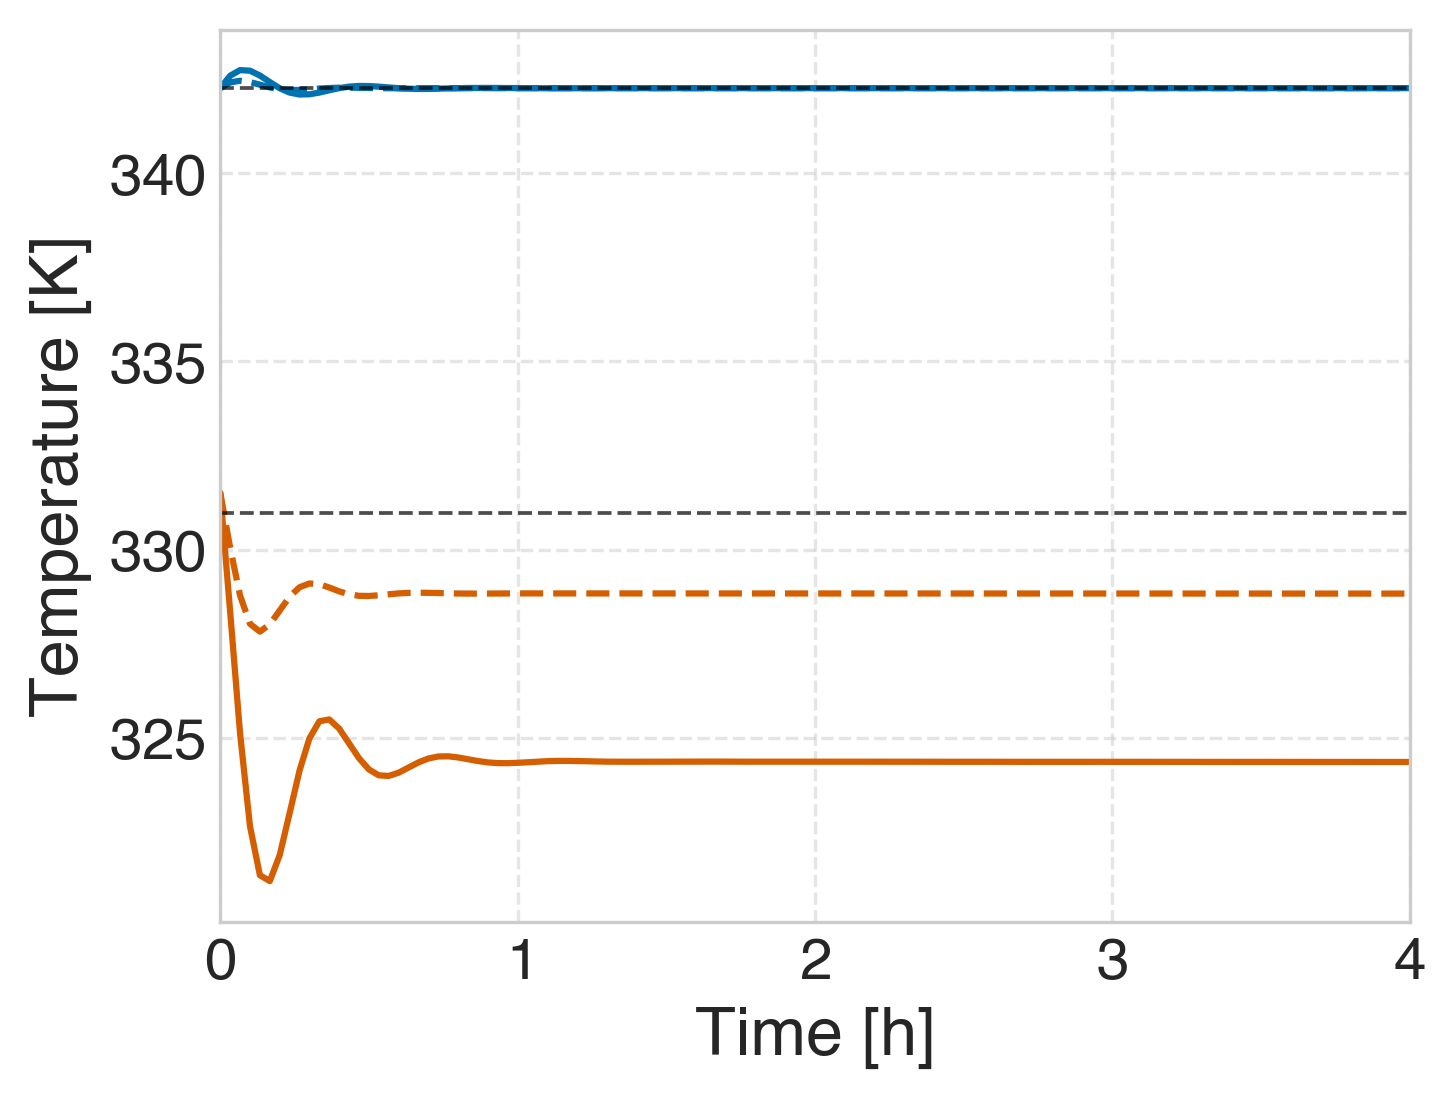
\includegraphics[width=0.9\linewidth]{nb21_cl_vs_ol_masking_2x1}
  \caption{Control masking in System~II under jacket fouling
    (noiseless). W5: $\beta_r=0.80$, dashed lines; W6: $\beta_r=0.60$, full lines. 
    Reactor temperature $T_r$ is shown in blue, jacket temperature $T_r$ in orange.
    \textit{Top:} Reactor temperature stays near the setpoint
    (dotted black line) under closed-loop operation regardless of fouling severity as Loop~1 masks the fault in the temperature channel. Jacket temperature $T_j$ drops proportionally to the
    fouling magnitude, providing
    the primary secondary observable for $\beta_r$.
    \textit{Bottom:} The open-loop trajectories
    (dashed) show the unmasked $T_r$ excursion that would be visible without
    feedback control. This is the same mechanism as the $\beta$ bias quantified
    for System~I (Section~\ref{sec:identifiability}), transferred exactly to the
    recycle plant.}
  \label{fig:wu_cl_masking}
\end{figure}
% ------------------------------------------------------------------

\subsection{Fault Scenarios and Parameterisation}
\label{sec:fault_params2}

Five independent multiplicative degradation factors are inferred from process observations (Table~\ref{tab:wu_fault_params}). The two reactor-side parameters ($\alpha$, $\beta_r$) from System~I plus three parameters to capture column and feed degradation: $\eta_\mathrm{col}$, $\xi_\mathrm{reb}$,  and $z_{A0,\mathrm{eff}}$. The first four parameters are multiplicative factors on the nominal physical constants, while $z_{A0,\mathrm{eff}}$ is an effective fresh-feed A fraction that accounts for variability
in the feed composition or upstream separation efficiency. The lower bound $\eta_\mathrm{col} \geq 0.80$ is imposed by numerical stability of the quasi-steady-state column shortcut.

% ------------------------------------------------------------------
\begin{table*}[htbp]
\centering
\caption{Fault parameters for System~II (Wu 2003 recycle plant). All parameters
  equal 1.0 at clean-service nominal conditions. The physical design constants
  $U\!A_r$ and $U\!A_\mathrm{reb}$ are treated as known and only the relative
  degradation factors are inferred.}
\label{tab:wu_fault_params}
\small
\begin{tabular}{clll}
\toprule
Symbol & Physical meaning & Prior & Primary observable \\  
\midrule
$\alpha$ & Catalyst activity factor & $\mathcal{U}(0.4,\,1.2)$ & $F_{R,\mathrm{norm}}$, $Q_j$ \\
$\beta_r$ & Reactor jacket conductance factor & $\mathcal{U}(0.4,\,1.2)$ & $T_j$, $Q_j$ \\
$\eta_\mathrm{col}$ & Column tray efficiency factor & $\mathcal{U}(0.80,\,1.0)$ & $T_\mathrm{reb}$, $Q_\mathrm{reb}$ \\
$\xi_\mathrm{reb}$ & Reboiler conductance factor & $\mathcal{U}(0.4,\,1.2)$ & $Q_\mathrm{reb}$ \\
$z_{A0,\mathrm{eff}}$ & Effective fresh-feed A fraction & $\mathcal{U}(0.70,\,0.95)$ & All channels via reactor SS \\
\bottomrule
\end{tabular}
\end{table*}
% ------------------------------------------------------------------

Incorporating all five degradation factors, the complete reactor--column--recycle
model replaces Eqs.~\eqref{eq:wu_reactor} and \eqref{eq:wu_recycle} with
%
\begin{subequations}
\label{eq:wu_degraded}
\begin{align}
  \frac{dz_A}{dt}
    =& \frac{F_\mathrm{in}}{M_r}\bigl(z_{A,\mathrm{in}} - z_A\bigr)
       - \alpha\,k(T_r)\,z_A,
  \label{eq:wu_dza_degraded} \\[4pt]
  \frac{dT_r}{dt}
    =& \frac{F_\mathrm{in}}{M_r}\bigl(T_\mathrm{in,mix} - T_r\bigr)
       + \frac{-\Delta H_r}{\rho C_p}\,\alpha\,k(T_r)\,z_A \nonumber \\
     & - \frac{\beta_r\,U\!A_r}{\rho C_p V_r}\bigl(T_r - T_j\bigr),
  \label{eq:wu_dtr_degraded} \\[4pt]
  \frac{dT_j}{dt}
    =& \frac{\beta_r\bigl[U\!A_r(T_r - T_j) - Q_j\bigr]}{M_j\,C_{pj}},
  \label{eq:wu_dtj_degraded}
\end{align}
\end{subequations}
%
where the fresh-feed composition fault propagates through the feed-mixing relation
%
\begin{equation}
  z_{A,\mathrm{in}} = \frac{F_0\,z_{A0,\mathrm{eff}} + F_R\,x_D}{F_\mathrm{in}},
  \qquad
  T_\mathrm{in,mix} = \frac{F_0\,T_\mathrm{in} + F_R\,T_r}{F_\mathrm{in}},
  \label{eq:wu_zain_degraded}
\end{equation}
%
replacing the healthy-feed value $z_0 = 0.90$ of Eq.~\eqref{eq:wu_recycle} by the inferred effective composition $z_{A0,\mathrm{eff}}$.  The column tray-efficiency
factor $\eta_\mathrm{col}$ scales the effective relative volatility away from its clean-service value, Eq.~\eqref{eq:wu_alphaeff},
%
\begin{equation}
  \alpha_\mathrm{eff} = 1 + \eta_\mathrm{col}\,(\alpha_\mathrm{rel} - 1),
  \label{eq:wu_alphaeff_degraded}
\end{equation}
%
which sets $x_D$, $x_B$, and hence the recycle flow $F_R$ appearing in Eqs.~\eqref{eq:wu_dza_degraded} and \eqref{eq:wu_zain_degraded}.  Finally, the
reboiler conductance factor $\xi_\mathrm{reb}$ scales the heat duty that Loop~3 must supply to hold the column material balance at its quasi-steady state,
%
\begin{equation}
  Q_\mathrm{reb} = \frac{Q_{\mathrm{reb,nom}}}{\xi_\mathrm{reb}}\cdot
    \frac{F_\mathrm{in}}{F_{\mathrm{in,nom}}}\cdot V_\mathrm{norm},
  \label{eq:wu_qreb_degraded}
\end{equation}
%
where $F_{\mathrm{in,nom}} = F_0 + F_{R,\mathrm{nom}}$ and $V_\mathrm{norm}$ is the normalised boilup effort commanded by Loop~3. A fouled reboiler ($\xi_\mathrm{reb} < 1$) therefore requires a proportionally larger duty $Q_\mathrm{reb}$ for the same throughput and boilup effort which is directly analogous to the role of $\beta_r$ in the reactor jacket balance, Eq.~\eqref{eq:wu_dtj_degraded}.

Table~\ref{tab:si_wu_scenarios} lists the fourteen closed-loop fault scenarios studied through 30 stochastic replicates each giving rise to 420 observation windows. The scenarios cover individual single-parameter faults, compound multi-parameter faults, and a near-snowball-tipping-point scenario.  
%Full scenario definitions are provided in Table~S2 of the Supporting Information.
Data generation follows the same Euler--Maruyama protocol as System~I, adapted to 2-hour windows at 1-min sampling resolution (120 time steps). The process-noise levels and training hyperparameters are detailed in Section~S7 of the Supporting Information.

% ------------------------------------------------------------------
\begin{table*}[htbp]
\centering
\caption{Fault scenario catalogue for System~II. All scenarios use 30 independent
  stochastic replicates per control structure, each comprising a 2-hour observation
  window at 1-min sample interval (120 time steps). Parameters equal 1.0 unless
  otherwise listed.}
\label{tab:si_wu_scenarios}
\small
\begin{tabular}{cllcccccl}
\toprule
ID & Name & Fault unit & $\alpha$ & $\beta_r$ & $\eta_\mathrm{col}$ & $\xi_\mathrm{reb}$ & $z_{A0}$ & Primary purpose \\
\midrule
W1  & Healthy nominal     & Healthy  & 1.00 & 1.00 & 1.00 & 1.00 & 0.90 & SBI training / baseline \\
W2  & Cat.~decay mild     & Reactor  & 0.90 & 1.00 & 1.00 & 1.00 & 0.90 & Single-param: $\alpha$ \\
W3  & Cat.~decay severe   & Reactor  & 0.65 & 1.00 & 1.00 & 1.00 & 0.90 & Snowball onset \\
W4  & Cat.~near tipping   & Reactor  & 0.58 & 1.00 & 1.00 & 1.00 & 0.90 & Near snowball limit \\
W5  & Jacket fouling mild & Reactor  & 1.00 & 0.80 & 1.00 & 1.00 & 0.90 & Single-param: $\beta_r$ \\
W6  & Jacket fouling severe& Reactor & 1.00 & 0.60 & 1.00 & 1.00 & 0.90 & Single-param: $\beta_r$ \\
W7  & Col.~eff.~mild      & Column   & 1.00 & 1.00 & 0.90 & 1.00 & 0.90 & Single-param: $\eta_\mathrm{col}$ \\
W9  & Reboiler fouling    & Column   & 1.00 & 1.00 & 1.00 & 0.80 & 0.90 & Single-param: $\xi_\mathrm{reb}$ \\
W10 & Feed purity drop    & Feed     & 1.00 & 1.00 & 1.00 & 1.00 & 0.75 & Single-param: $z_{A0}$ \\
W11 & Cat.~+ jacket       & Reactor  & 0.80 & 0.80 & 1.00 & 1.00 & 0.90 & Compound: reactor faults \\
W12 & Cat.~+ col.~eff.    & Multi    & 0.75 & 1.00 & 0.80 & 1.00 & 0.90 & Compound: cross-unit \\
W13 & Cat.~+ feed         & Multi    & 0.80 & 1.00 & 1.00 & 1.00 & 0.80 & Compound: reactor + feed \\
W15 & Cat.~+ col.~mild    & Multi    & 0.75 & 1.00 & 0.90 & 1.00 & 0.90 & Near tipping + column \\
W16 & Full multi-fault    & Multi    & 0.80 & 0.85 & 0.90 & 0.85 & 0.85 & All-unit degradation \\
\bottomrule
\end{tabular}
\end{table*}
% ------------------------------------------------------------------

% =============================================================================
\section{Inference Methodology}\label{sec:methodology}
% =============================================================================

The inference framework applied in this work is known as \emph{simulation-based inference} (SBI), a likelihood-free inference methodology used when the likelihood function $p(\mathbf{y} \mid \boldsymbol{\theta})$ is analytically intractable or unavailable, but simulation of synthetic data $\mathbf{y}_\text{sim} \sim p(\mathbf{y} \mid \boldsymbol{\theta})$ is feasible \citep{Cranmer2020}. This methodology is widely used in scientific applications where the underlying physical model is known, but the complexity of the system makes it difficult to derive a closed-form expression for the likelihood
%(Section~\ref{sec:related_work} positions this work against the one prior
%application of SBI to chemical-process equipment monitoring, \citet{Collett2026}).
In such cases, SBI allows for the estimation of posterior distributions over model parameters by leveraging simulations to generate synthetic datasets that can be compared to observed data. This approach is well-suited to the closed-loop fault diagnosis problem, where the feedback complicates the likelihood function.

The applied SBI framework comprises three successive stages: (i)~A JAX-vectorised stochastic simulator that generates synthetic observation windows from the degraded closed-loop models. (ii)~An amortised neural posterior estimator trained to approximate the Bayesian posterior $p(\boldsymbol{\theta}\mid\mathbf{s})$ over the degradation-parameter vector $\boldsymbol{\theta}$ given any realisation of the summary statistics. (iii)~A threshold-and-unit-aggregation rule (Section~\ref{sec:fault_class}) that maps the joint posterior to a discrete fault class, reducing to four non-overlapping quadrants of the fault-parameter space for System~I and to five unit-level classes for System~II. The inference methodology is identical across System~I (Section~\ref{sec:system1}) and System~II
(Section~\ref{sec:system2}) and differ only in the dimensionality of $\boldsymbol{\theta}$, the summary statistics $\mathbf{s}$, and the density-estimator training configuration (hyper parameters).
The framework is implemented in the \texttt{sbi} library~\citep{Tejero_cantero_3be1efca,BoeltsDeistler_sbi_2025}.
Following the notation of \citet{Cranmer2020}, the estimator is operated in the \emph{amortised} regime: the simulator is only queried at training time, and subsequent
inference on any new 60-minute window requires only a single forward pass through the trained network, with typical latency below 20~ms.
%The three stages are described in detail below.


\subsection{Amortised Posterior Estimation and Classification}
\label{sec:sbi_method}
% ---------------------------------------------------------------------------

%\subsubsection{Prior distribution and inference target}
The inference target is an $n$-dimensional degradation-parameter vector $\boldsymbol{\theta}=(\theta_1,\ldots,\theta_n)$, with each component
assigned an independent uniform prior distribution:
%
\begin{equation}
  p(\boldsymbol{\theta}) =
  \bigotimes_{j=1}^{n}
  \mathcal{U}\!\bigl([\theta_{j,\mathrm{lo}},\,\theta_{j,\mathrm{hi}}]\bigr).
  \label{eq:prior}
\end{equation}
%
For System~I, $n=2$ and $\boldsymbol{\theta}=(\alpha,\beta)$, both assigned
$\mathcal{U}(0.4,\,1.2)$ (Table~\ref{tab:params_system1}). For System~II,
$n=5$ and
$\boldsymbol{\theta}=(\alpha,\beta_r,\eta_\mathrm{col},\xi_\mathrm{reb},z_{A0,\mathrm{eff}})$,
with per-parameter bounds given in Table~\ref{tab:wu_fault_params}.
For the parameters shared across both systems which are centred on a healthy value of 1 ($\alpha$; $\beta$ or $\beta_r$; $\xi_\mathrm{reb}$), the upper bound of 1.2 serves dual purpose: it allows for a small positive bias in the estimated parameters, and it provides a numerical buffer around the healthy operating point, preventing the density estimator from being trained against a hard boundary at the most frequently sampled condition. The remaining two System~II parameters have bounds set by other constraints (Table~\ref{tab:wu_fault_params}): $\eta_\mathrm{col}$'s lower bound of 0.80 is set by the numerical stability of the quasi-steady-state column shortcut (Section~\ref{sec:fault_params2}), and $z_{A0,\mathrm{eff}}$'s bounds are centred on its own healthy value of 0.90, not 1.

A conditional density estimator $q_\phi(\boldsymbol{\theta}\mid\mathbf{s})$ is trained by minimising the expected forward Kullback--Leibler divergence over simulated $(\boldsymbol{\theta},\mathbf{s})$ pairs drawn from the joint prior-predictive distribution,
%
\begin{equation}
  \mathcal{L}(\phi)
  \;=\;
  -\,\mathbb{E}_{p(\boldsymbol{\theta})\,p(\mathbf{y}\mid\boldsymbol{\theta})}
  \!\Bigl[
    \log q_\phi\!\bigl(\boldsymbol{\theta}\mid\mathbf{s}(\mathbf{y})\bigr)
  \Bigr].
  \label{eq:snpe_loss}
\end{equation}
%
Where $\mathbf{s}(\mathbf{y})$ is the summary statistic vector extracted from the raw observation window $\mathbf{y}$, and $p(\mathbf{y}\mid\boldsymbol{\theta})$ 
is the stochastic simulator (Section~\ref{sec:scenarios}). The expectation is approximated by Monte Carlo sampling of $(\boldsymbol{\theta},\mathbf{y})$ pairs from the prior and simulator, and the loss is minimised with respect to the density-estimator parameters $\phi$ using stochastic gradient descent. The trained estimator $q_\phi$ thus approximates the Bayesian posterior $p(\boldsymbol{\theta}\mid\mathbf{s})$ for any summary statistic vector $\mathbf{s}$ reachable under the prior, enabling
deployment on any new observation window without retraining.

This is the single-round amortised formulation of sequential neural posterior estimation~\citep[SNPE-C;][]{Greenberg2019}, in which the proposal distribution coincides with the prior so that no importance correction is required.  The estimator $q_\phi$ thus approximates the Bayesian posterior $p(\boldsymbol{\theta}\mid\mathbf{s})$ jointly for all summary statistics reachable under the prior, enabling deployment on any new observation window within the same distribution without retraining.

%\paragraph{Relation to the direct method of closed-loop identification.}
Following \citet{Forssell1999}, SNPE-C operates on the measured signal histories $\mathbf{x}(t)$ without requiring an explicit model of the feedback controller, making it a probabilistic analogue of the \emph{direct method} of closed-loop system identification. Like the classical direct approach, it is universally applicable to nonlinear and
saturating feedback and exploits the persistent in-loop process noise to partially recover parameter information that is structurally reduced by integral action~\citep{Ljung1999}.

The conditional distribution $q_\phi(\theta\vert{}s)$ is parameterised by a neural spline flow~\citep{Durkan2019}. Network architectures, training budgets ($n_{sim} = 10,000$ for System I; $15,000$ for System II), and ensembling strategies were independently validated for each system to ensure optimal posterior calibration while avoiding over-parameterisation.  Full details of the network architectures, hyperparameter sweeps, and seed-stability strategies are provided in the Supporting Information (Sections S3 and S7.3).

Posterior calibration is assessed using simulation-based calibration~\citep{Talts2018}, which tests whether the rank of the true parameter among posterior draws is uniformly
distributed across independent test cases drawn from the prior. The full protocol, acceptance criteria, and rank histograms for each system's production posterior are
given in the Supporting Information (Section~S6, System~I; Section~S9.2, System~II).

\phantomsection\label{sec:fault_class}
The joint posterior $q_\phi(\boldsymbol{\theta}\mid\mathbf{s})$ is mapped to a discrete fault class by a two-level rule applied uniformly to both systems. First, each degradation parameter $\theta_j$ is compared against a relative threshold $\theta_\mathrm{thr}=0.85$ (a 15\% reduction relative to its clean-service baseline) and flagged as degraded if $\theta_j<\theta_\mathrm{thr}$. For System~II, $z_{A0,\mathrm{eff}}$ is flagged relative to its own healthy value of 0.90, since a feed-purity fault is one-sided (always a reduction, never an increase). Second, parameters are grouped into physical units such that for System~I, each of the two parameters is its own unit; while for System~II, reactor $=\{\alpha,\beta_r\}$, column $=\{\eta_\mathrm{col},\xi_\mathrm{reb}\}$, feed $=\{z_{A0,\mathrm{eff}}\}$. A unit is flagged degraded if any of its member parameters is degraded. The reported class is the combination of degraded units with the greatest posterior mass: \emph{healthy} (no unit degraded), the corresponding unit label if exactly one unit is degraded, or \emph{multi} %(System~II) / \emph{combined} (System~I) 
if more than one unit is degraded simultaneously. The associated confidence is given by the posterior mass assigned to the reported class. For System~I, with two parameters each forming its own unit, this reduces to four non-overlapping quadrants of the $(\alpha,\beta)$ plane: \emph{healthy}, \emph{fouling-dominant}, \emph{decay-dominant}, and \emph{multi}. For System~II it produces five classes (healthy, reactor, column, feed, multi), detailed in Section~\ref{sec:wu_fault_class}. The 0.85 threshold corresponds to a 15\% reduction in the effective rate constant or conductance relative to the clean-service baseline for the reactor- and column-side parameters ($\alpha$, $\beta$/$\beta_r$, $\eta_\mathrm{col}$, $\xi_\mathrm{reb}$), exceeding typical run-to-run variability and providing a meaningful trigger for maintenance decisions. For the feed-purity parameter $z_{A0,\mathrm{eff}}$, the same relative threshold instead flags a compositional deviation rather than a rate-constant or heat-transfer-coefficient reduction.

% =============================================================================
%  Nomenclature entries (to be collected into a common \nomenclature block)
% =============================================================================
%
%  \nomenclature{$C$}{Propylene oxide concentration in the reactor, mol~L$^{-1}$}
%  \nomenclature{$T$}{Reactor temperature, K}
%  \nomenclature{$T_c$}{Jacket temperature, K}
%  \nomenclature{$I$}{Anti-windup PI integrator state, K~min}
%  \nomenclature{$Q_c$}{Coolant volumetric flow rate, L~min$^{-1}$}
%  \nomenclature{$k(T)$}{Reaction rate constant at temperature $T$, min$^{-1}$}
%  \nomenclature{$k_0$}{Pre-exponential (Arrhenius) factor, min$^{-1}$}
%  \nomenclature{$E_a$}{Activation energy, J~mol$^{-1}$}
%  \nomenclature{$\Delta H_r$}{Standard enthalpy of reaction, J~mol$^{-1}$}
%  \nomenclature{$R$}{Universal gas constant, J~(mol~K)$^{-1}$}
%  \nomenclature{$U\!A$}{Overall heat transfer coefficient-area product, cal~(min~K)$^{-1}$}
%  \nomenclature{$V$}{Reactor volume, L}
%  \nomenclature{$V_c$}{Jacket volume, L}
%  \nomenclature{$Q$}{Volumetric feed flow rate, L~min$^{-1}$}
%  \nomenclature{$\rho$}{Reactor fluid density, g~L$^{-1}$}
%  \nomenclature{$C_p$}{Reactor fluid heat capacity, cal~(g~K)$^{-1}$}
%  \nomenclature{$\alpha$}{Catalyst activity degradation factor, dimensionless}
%  \nomenclature{$\beta$}{Jacket conductance degradation factor, dimensionless}
%  \nomenclature{$K_p$}{PI proportional gain, (L~min$^{-1}$)~K$^{-1}$}
%  \nomenclature{$\tau_i$}{PI integral time constant, min}
%  \nomenclature{$T_\mathrm{sp}$}{Reactor temperature setpoint, K}

% =============================================================================
\section{Results: System~I --- Propylene Oxide CSTR}
\label{sec:results_system1}
% =============================================================================

% ---------------------------------------------------------------------------
\subsection{Physics-Informed Summary Statistics}
\label{sec:summary_stats}
% ---------------------------------------------------------------------------

Each replicate observation window $\mathbf{x}\in\mathbb{R}^{120\times4}$ is compressed to a 29-dimensional summary-statistic vector $\mathbf{s}(\mathbf{x})\in\mathbb{R}^{29}$ prior to passing it to the density estimator. The 29 features are organised into four groups, each motivated by a distinct facet of the closed-loop fault-diagnosis problem (Table~S1 of the Supporting Information). 27 of the features are standard time-series descriptors (e.g., moments, trends) and control-effort aggregates while the remaining two features are explicitly target the degradation parameters. They are derived by algebraic inversion of the closed-loop steady-state balance equations, making them direct proxies for the identifiable parameter products $\beta\!\cdot\!U\!A$ and$\alpha\!\cdot\!k_0$:
%
\begin{align}
  s_{U\!A} &= \frac{\bar{T}-\bar{T}_c}{\bar{Q}_c},
  \label{eq:ua_proxy}\\[4pt]
  s_{k_0} &= \ln\!\left(\frac{\bar{C}}{C_i - \bar{C}}\right),
  \label{eq:k0_proxy}
\end{align}
%
where $\bar{(\cdot)}$ denotes the whole-window mean of the respective channel. Under non-saturating PI control at steady state, $s_{U\!A}\propto(\beta\!\cdot\!U\!A)^{-1}$ follows from the jacket energy balance, and $s_{k_0}\propto(\alpha\!\cdot\!k_0)^{-1}$ follows from the component balance at fixed conversion. Used alone, these two features achieve 98.3\% cross-validated Linear Discriminant Analysis (LDA) \citep{Zhou2021} accuracy on the eight-scenario dataset, confirming that they encode nearly all of the identifiable information about $(\alpha,\beta)$ accessible from stationary, noise-free steady-state observations. Figure~\ref{fig:physics_scatter} illustrates
this separation directly as all eight scenarios occupy well-separated,
compact clusters in the $(s_{U\!A},\,s_{k_0})$ plane.

% ------------------------------------------------------------------
\begin{figure}[htbp]
  \centering
  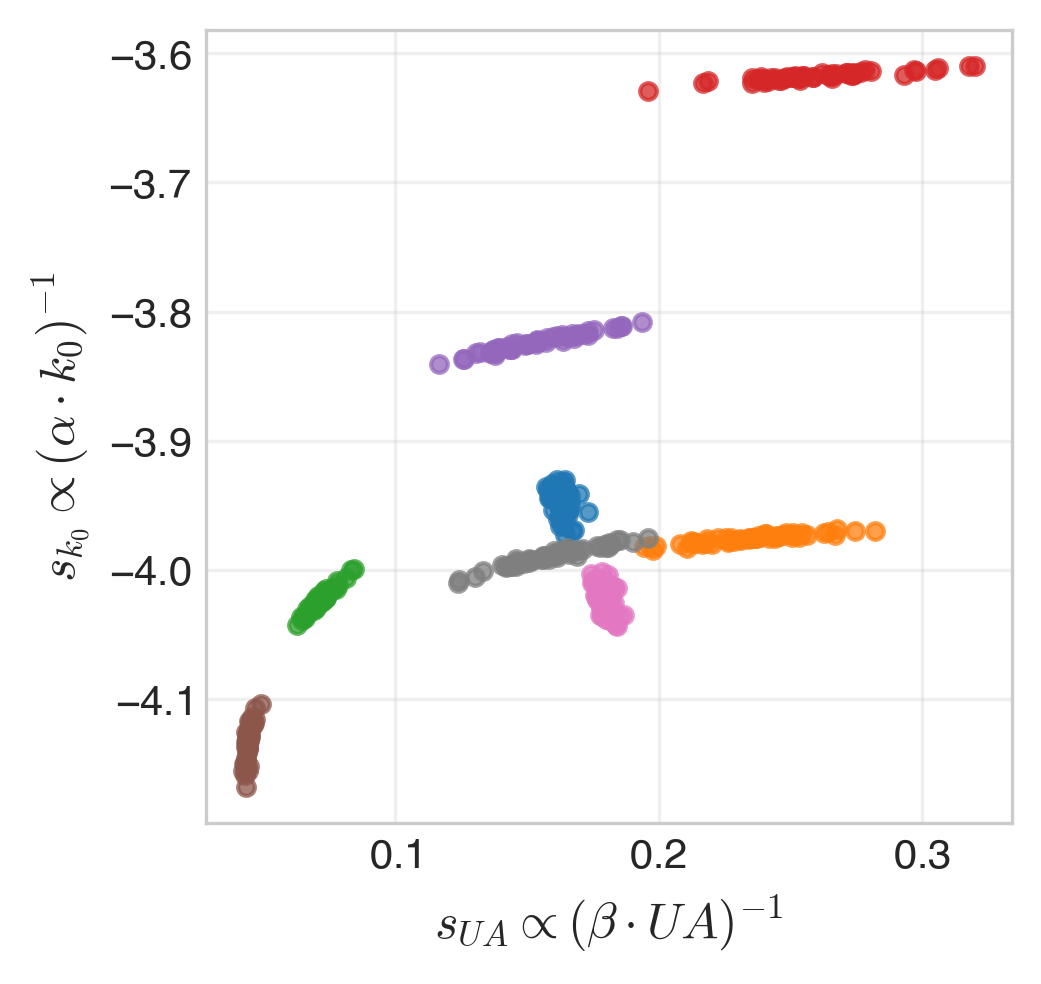
\includegraphics[width=0.97\linewidth]{03_physics_features_scatter}
  \caption{Scenario separation in the two physics-informed summary
    features. Each point represents one of the 50 stochastic
    replicates with colour indicating scenario (Sc0-Sc7). The $x$-axis encodes
    $s_{U\!A} \propto (\beta\!\cdot\!U\!A)^{-1}$, the $y$-axis encodes
    $s_{k_0} \propto (\alpha\!\cdot\!k_0)^{-1}$. The eight scenarios
    occupy distinct, nearly non-overlapping clusters, confirming that
    the 2-D physics-proxy subspace encodes almost all identifiable
    information about $(\alpha,\beta)$ at steady state. Scatter within
    each cluster is due to process and sensor noise.}
  \label{fig:physics_scatter}
\end{figure}
% ------------------------------------------------------------------

In the noise-free stationary limit, $s_{U\!A}$ and $s_{k_0}$ alone suffice for exact identification of $(\alpha,\beta)$. The 25 additional features are required for robustness under noise amplification in the proxy ratio, transient dynamics during fault onset, actuator saturation (Sc\,5), and open-loop windows where $Q_c$ is constant. 

% ---------------------------------------------------------------------------

% ---------------------------------------------------------------------------
\subsection{Training Validation and Fault Classification}
\label{sec:snapshot_classification}
% ---------------------------------------------------------------------------
Simulator coverage of the evaluation regime was confirmed through prior predictive checks over 500 parameter vectors drawn from the prior, spanning the observed data range for all 29 summary features across every closed-loop scenario ~\citep{Cranmer2020} (Fig.~S1 of the Supporting
Information). Posterior calibration with 500 test cases rejected rank uniformity at the 5\% level (Kolmogorov-Smirnov (KS) $p$-values of $0.016$ for $\alpha$ and $0.014$ for $\beta$). The two-sample classifier scores of 0.52 and 0.53 are near the uninformative baseline of 0.5 which indicating that the deviation reflects structural information deficit rather than a training deficiency. Rank histograms and
full interpretation are given in Supporting Information Section~S6.

Five-fold stratified cross-validated LDA confirmed the fill 29-D vector achieves 100\% scenario-classification accuracy versus 98.3\% for the physics-2
subset alone (Principal Component Analysis (PCA) 
and features in Figures~S3 and Tables~S1--S2 of the Supporting Information).
The trained NSF posterior applied 400 evaluation windows (8 scenarios, 50 replicates each) with $\theta_\mathrm{thr}=0.85$ yielded macro-$F_1 = 0.990$
across the six closed-loop scenarios (Sc\,1--5, Sc\,7).
Perfect classification ($F_1 = 1.0$) was achieved for the healthy scenario (Sc\,1), jacket fouling (Sc\,2), and catalyst decay (Sc\,3).
The multi-fault scenario (Sc\,4,$\alpha^*=\beta^*=0.85$) attained 
$F_1 = 0.94$ with misclassifications arising from the noise pushing posterior mass across the threshold.  Quantitative per-scenario results are summarised in
Table~\ref{tab:scenario_results} and in Figure~\ref{fig:posterior_recovery}.
\begin{figure}[tb]
  \centering
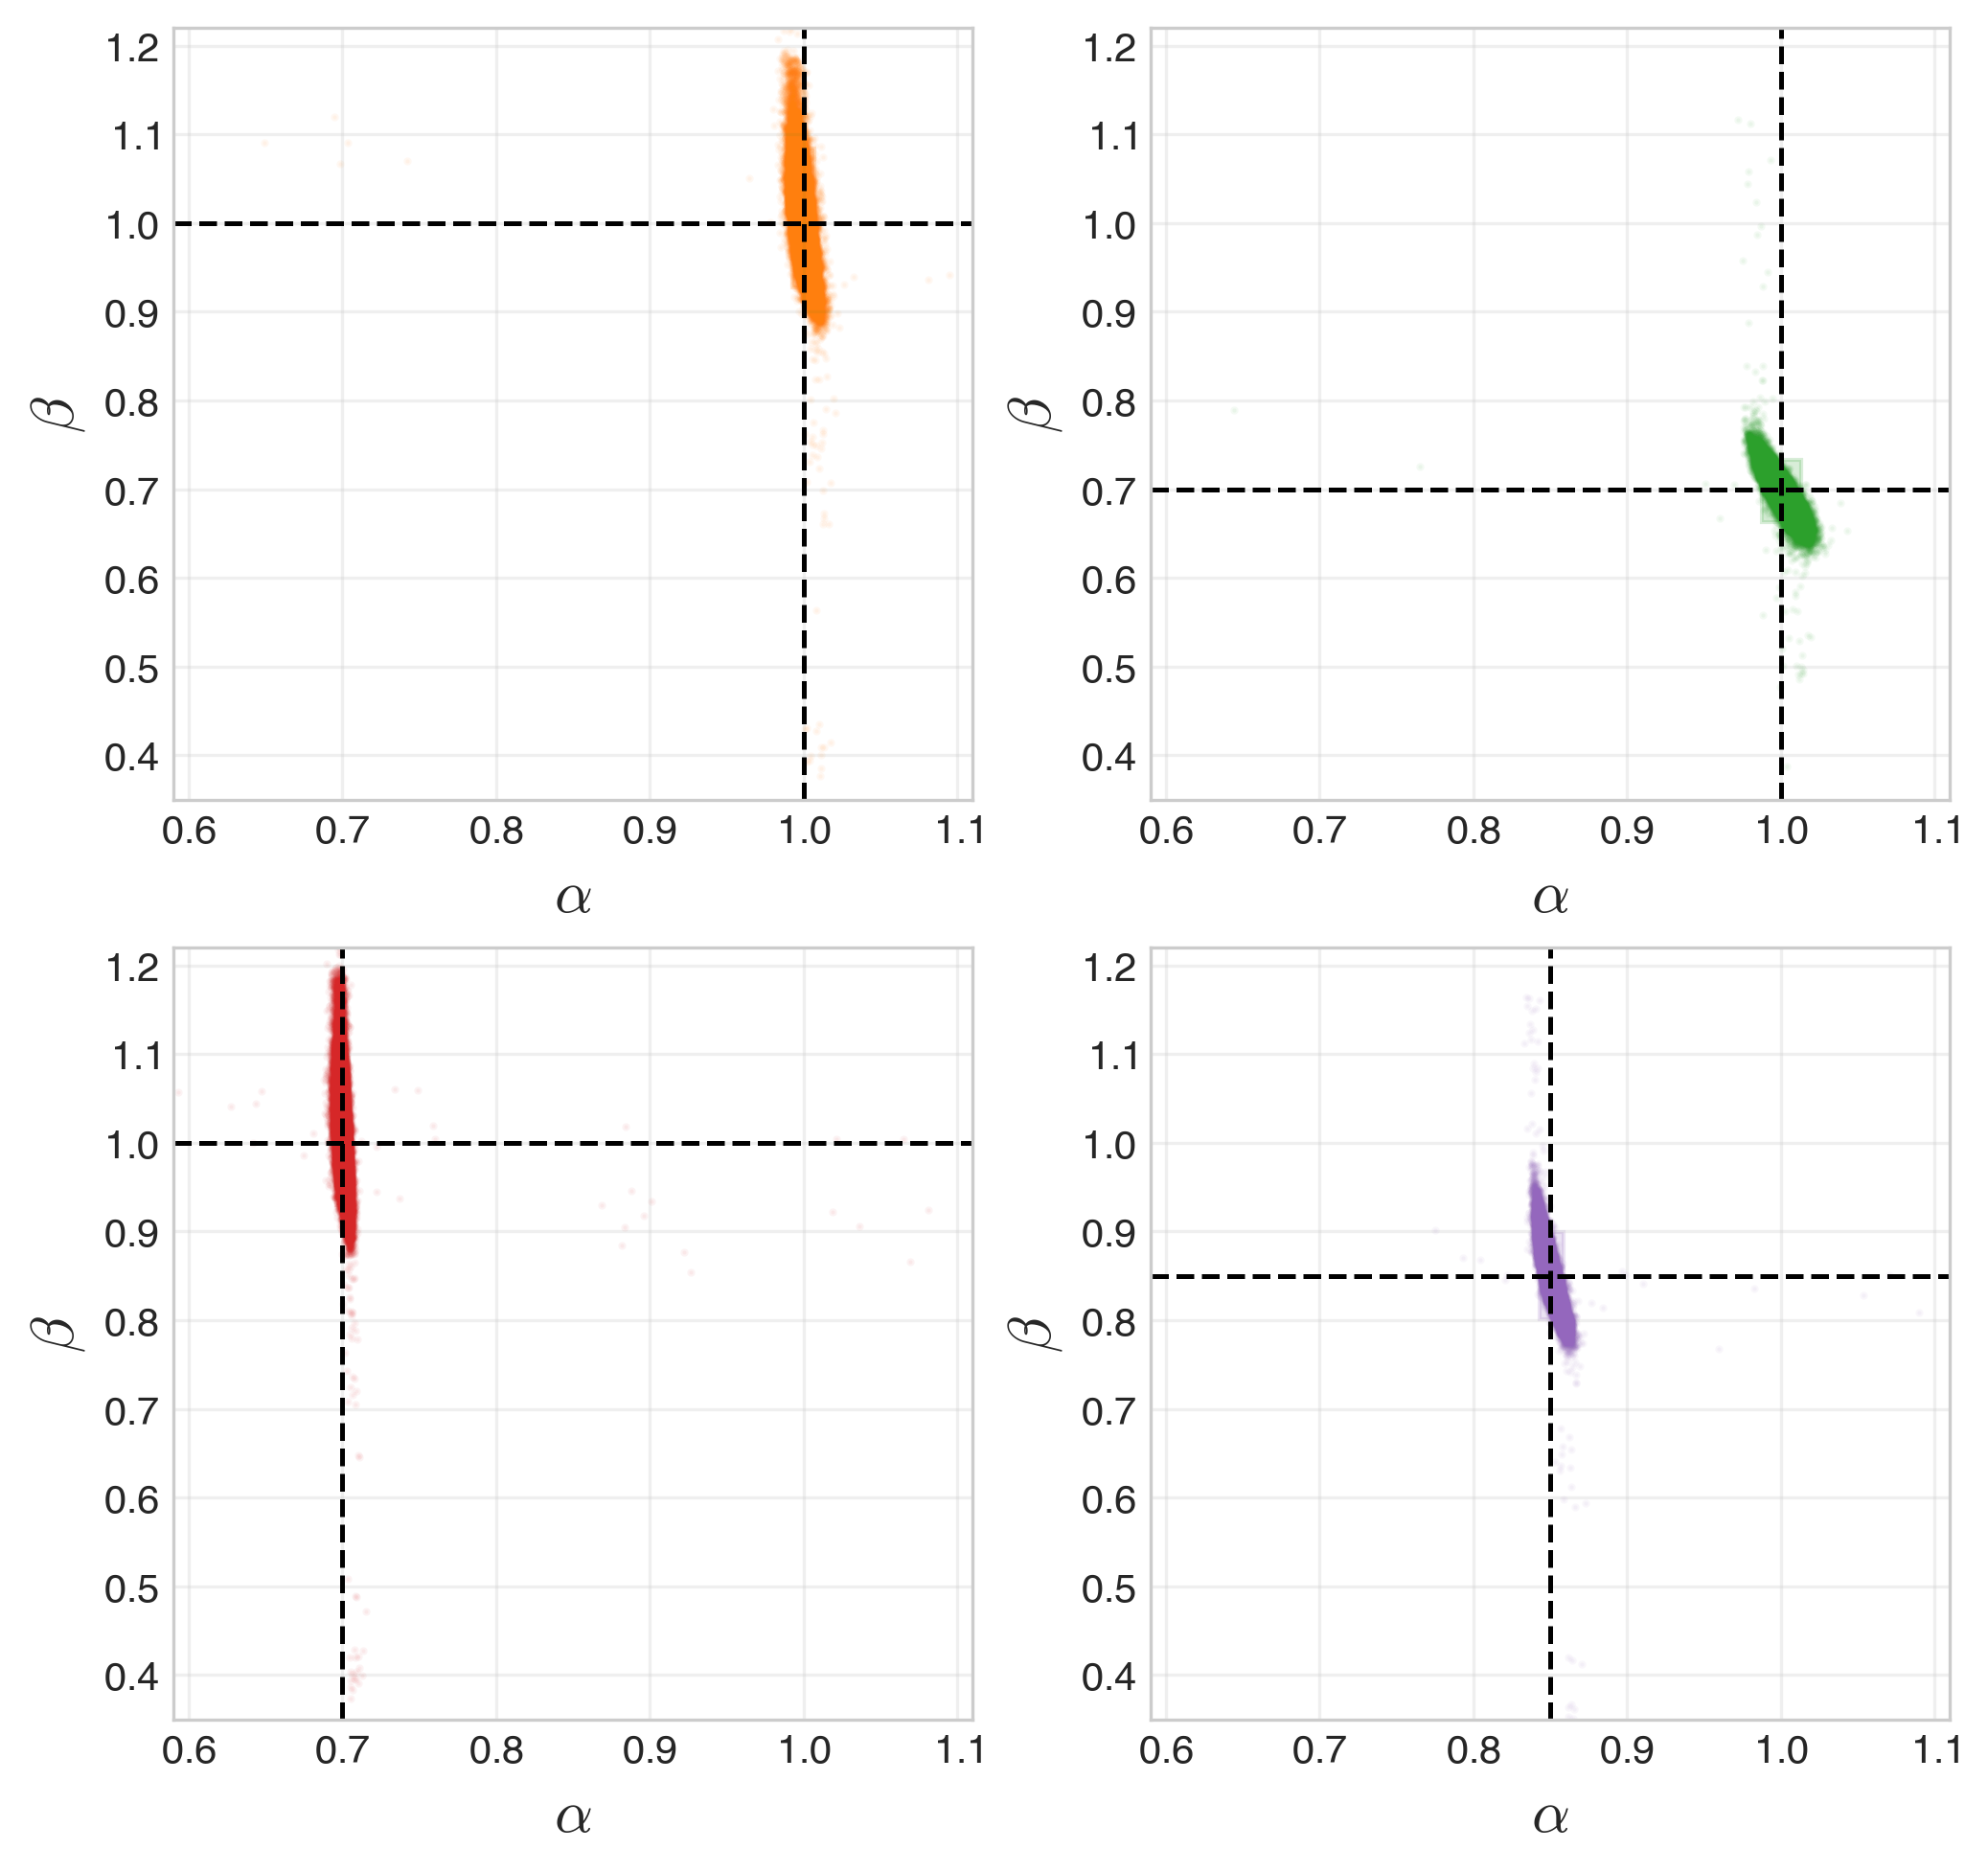
\includegraphics[width=0.95\linewidth]{06_joint_posterior_primary.png}
  \caption{Joint posterior samples for the primary System I closed loop scenarios: Sc1 (normal operation, orange), Sc2 (fouling, green), Sc3 (catalyst decay, red), Sc4 (combined, purple). 
  Each panel pools posterior samples for one scenario and plots the inferred degradation parameters $\alpha$ and $\beta$. 
  Dashed black lines mark the true scenario values. The narrow vertical structure of the posteriors indicates that $\alpha$ is generally tightly constrained, while $\beta$ varies more strongly across the fault scenarios.}\label{fig:posterior_recovery}
\end{figure}
% ------------------------------------------------------------------
%\begin{figure*}[htbp]
%  \centering
%  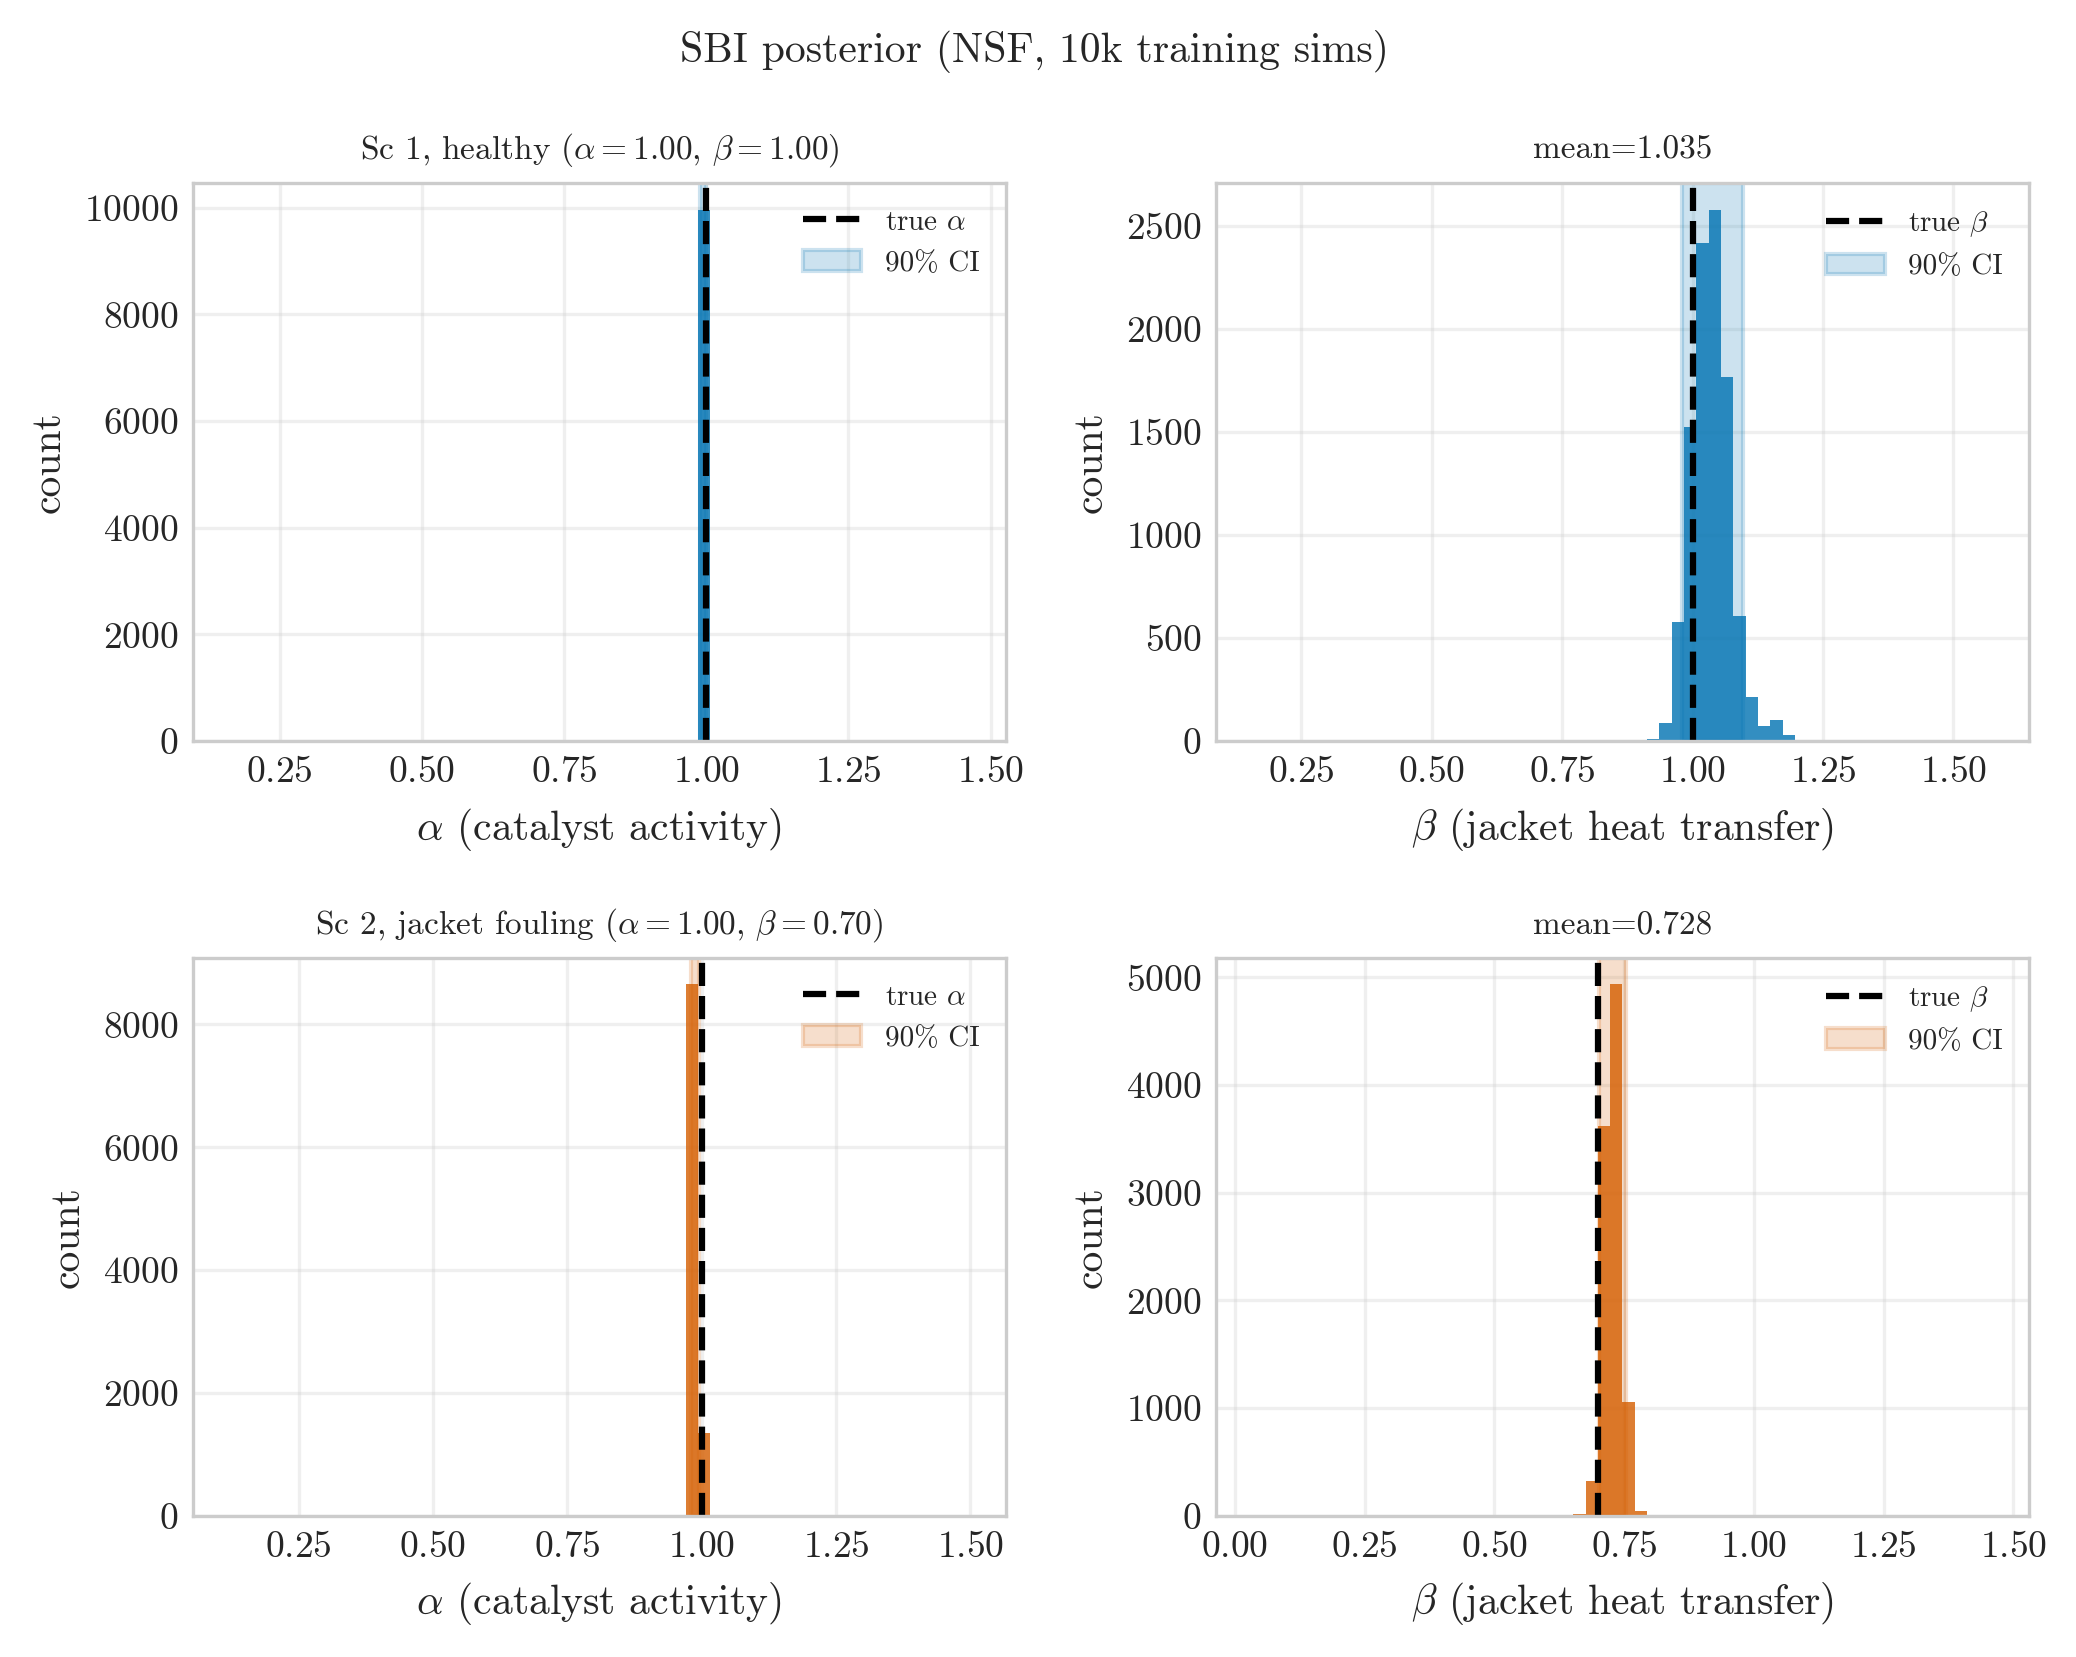
\includegraphics[width=0.97\linewidth]{04_posterior_recovery}
%  \caption{Posterior recovery for the healthy scenario (Sc\,1, top %row)
%    and the jacket-fouling scenario (Sc\,2, bottom row). Each panel
%    shows the marginal histogram of 10{,}000 posterior samples from %the production NSF posterior applied to a single representative replicate.
 %   Dashed lines mark the true parameter values, shaded bands indicate the
  %  90\% credible interval. \textit{Left:} $\alpha$ marginal --- recovered
%    with negligible bias across both scenarios.  \textit{Right:} $\beta$
%    marginal --- recovered to within the 90\% CI for Sc\,1; the downward
%    bias of approximately $-0.08$ for Sc\,2 is the structural closed-loop
%    masking effect quantified in Section~\ref{sec:identifiability}.}
%  \label{fig:posterior_recovery}
%\end{figure*}
% ------------------------------------------------------------------

% ------------------------------------------------------------------
\begin{table*}[htbp]
\centering
\caption{System~1 per-scenario evaluation results for the production NSF
  posterior (50 replicates per scenario).  $\hat{\alpha}$
  and $\hat{\beta}$ are posterior means, 90\%~CI coverage gives the
  fraction of replicates for which the 90\% credible interval contains
  the true value, $F_1$ is the per-scenario fault-classification F\textsubscript{1}
  score.  Open-loop scenarios (Sc\,0, Sc\,6) are evaluated with a
  closed-loop-trained posterior and therefore reflect the mode-mismatch
  penalty discussed in Section~\ref{sec:model_mismatch_results}.}
\label{tab:scenario_results}
\small
\begin{tabular}{clccrrrr}
\toprule
ID & Name & $\alpha^*$ & $\beta^*$ &
$\hat{\alpha}$ & $\hat{\beta}$ & 90\%~CI $\beta$ & $F_1$ \\
\midrule
Sc\,0 & Open-loop healthy     & 1.00 & 1.00 & 0.99 & 1.01 & 0.90 & —\textsuperscript{a} \\
Sc\,1 & Closed-loop healthy   & 1.00 & 1.00 & 1.00 & 0.99 & 0.94 & 1.00 \\
Sc\,2 & Jacket fouling        & 1.00 & 0.70 & 1.00 & 0.62 & 0.92 & 1.00 \\
Sc\,3 & Catalyst decay        & 0.70 & 1.00 & 0.70 & 1.00 & 0.90 & 1.00 \\
Sc\,4 & Combined moderate     & 0.85 & 0.85 & 0.85 & 0.78 & 0.92 & 0.94 \\
Sc\,5 & Severe fouling        & 1.00 & 0.40 & 1.00 & 0.35 & 0.90 & 1.00 \\
Sc\,6 & Open-loop fault       & 1.00 & 0.70 & 1.00 & 0.90 & 0.22 & 0.08\textsuperscript{a} \\
Sc\,7 & Fouling + sensor drift & 1.00 & 0.85 & 1.01 & 0.79 & 0.90 & 0.92 \\
\midrule
\multicolumn{7}{l}{Macro-F1 (closed-loop scenarios only)} & \textbf{0.990} \\
\bottomrule
\end{tabular}
\begin{flushleft}
\textsuperscript{a} Evaluated with a closed-loop-trained posterior; open-loop
  mode mismatch is expected and intentional (see Section~\ref{sec:model_mismatch_results}).
\end{flushleft}
\end{table*}
% ------------------------------------------------------------------

%\paragraph{Closed-loop versus open-loop training mismatch.}
\phantomsection\label{sec:model_mismatch_results}
The mode-mismatch experiment (Sc\,2 evaluated with a posterior trained on
open-loop data) quantifies the inferential cost of ignoring the feedback
structure.  The open-loop-trained posterior yields a Wasserstein-1 distance
on $\beta$ of 0.578, compared with 0.149 for the matched closed-loop posterior, a degradation of 288\%.  The CRPS on $\beta$ increases by 334\%.  When the
situation is reversed (closed-loop-trained posterior applied to open-loop
observations, Sc\,6), fault classification accuracy collapses from 1.0 to 0.06 as
the closed-loop posterior assigns substantial mass above the $\beta = 0.85$
threshold because it has learned to interpret constant $Q_c$ trajectories
as evidence of healthy operation.  Neither direction of mismatch is
correctable within the single-round amortised framework where matched training
is a necessary condition.

% ---------------------------------------------------------------------------
\subsection{Structural Identifiability Analysis}
\label{sec:identifiability}
% ---------------------------------------------------------------------------

%\subsubsection{Fisher information asymmetry}
%\label{sec:fim_asymmetry}

The Fisher information matrix (FIM) $\mathbf{I}(\boldsymbol{\theta})$ at a given
operating point quantifies the maximum information the summary statistics carry
about each parameter~\citep{Rao1945} and it can be used to predict the asymptotic 
covariance of any unbiased estimator \citep{identifiability1990, identifiability2026}. 
This approach is widely used in the chemical engineering 
literature~\citep{Gevers2011,Bombois2006} to quantify the
identifiability of model parameters from noisy measurements, and it has been
applied to the CSTR system studied here by \citet{Forssell1999} 
Computed numerically as
$\mathbf{I} = \mathbf{J}^\mathsf{T}\boldsymbol{\Sigma}^{-1}\mathbf{J}$, where
$\mathbf{J}_{ij} = \partial\bar{s}_i/\partial\theta_j$ is the Jacobian of the
expected summary statistics and $\boldsymbol{\Sigma}$ is the diagonal noise
covariance estimated from healthy replicates, the matrix reveals a dramatic
asymmetry at the nominal operating point:
%
\begin{equation}
  \frac{I_{\alpha\alpha}}{I_{\beta\beta}} \approx \frac{850{,}000\text{--}975{,}000}{2{,}000\text{--}3{,}500} \approx 250\text{--}500\times.
  \label{eq:fim_ratio}
\end{equation}
%

This matrix has a geometric reading that recurs throughout the identifiability
analysis of both systems (Section~\ref{sec:wu_identifiability}). Its inverse
bounds the best achievable joint-uncertainty region for any pair of
parameters, visualised as an ellipse in parameter space.  A small, round
ellipse means both parameters are well and independently determined whereas a long,
thin, diagonal ellipse, a \emph{ridge}, means only some combination of
the two parameters is determined, not either one on its own.  The normalised
off-diagonal entry $I_{ij}/\sqrt{I_{ii}I_{jj}}$, used throughout
Sections~\ref{sec:wu_artifact1}--\ref{sec:wu_artifact3} to diagnose apparent
joint confounds in System~II, measures only the \emph{angle} of this
ellipse where 0 corresponds to a round, axis-aligned region, and $\pm1$ to a
degenerate ridge.

Angle alone is not sufficient evidence that a confound is genuine or
resolved, because a change of representation could in principle make the
ellipse rounder while also making it larger overall thereby reshuffling which
combination of parameters is uncertain without making either parameter more
precisely knowable in absolute terms.  This concern is sharpest when
comparing representations of very different dimension, as when a
66-dimensional whole-window summary is compared against a 360-dimensional
raw trajectory (Section~\ref{sec:wu_artifact2}). The remedy is the
Cram\'er-Rao bound itself: $\mathbf{I}^{-1}$ gives not just the ellipse's
angle but its actual \emph{size} expressed as the smallest possible variance any
unbiased estimator could achieve for each parameter, regardless of
inference method. A single-number summary of the ellipse's overall shape,
the \emph{condition number} of $\mathbf{I}$ (large when the ellipse is
nearly degenerate, close to unity when it is well-conditioned and round),
provides a numerical check that a shrinking off-diagonal reflects a
genuine improvement in achievable precision rather than an artefact of
comparing feature spaces of different size. Sections~\ref{sec:wu_artifact2}
and~\ref{sec:wu_artifact3} report this check alongside the normalised
off-diagonal for exactly this reason.

The per-channel decomposition explains the mechanism.  The $\alpha$
information budget is supplied primarily by the concentration channel
($\approx 60$\%) and the coolant flow channel ($\approx 40$\%), both of which
carry a strong Arrhenius sensitivity.  The $\beta$ budget, by contrast, is
drawn exclusively from the jacket temperature $T_c$ and $Q_c$ channels. The
reactor temperature $T$ contributes exactly zero because the PI controller
enforces $T_\mathrm{ss} = T_\mathrm{sp}$, making $\partial T_\mathrm{ss}/\partial\beta \equiv 0$.
These channels are substantially noisier and less sensitive to $\beta$ than
$C$ is to $\alpha$, producing the 250--500$\times$ deficit. The ratio is
consistent across all tested operating points and increases with proportional gain $K_p$ such that a tighter controller makes $\beta$ identification harder.

%\subsubsection{Analytical mechanism}
%\label{sec:analytical_mechanism}

Under non-saturating steady-state PI control ($T_\mathrm{ss} = T_\mathrm{sp}$),
the component balance decouples: $C_\mathrm{ss}$ depends on $\alpha$ only,
through the effective rate constant $\alpha k_0 e^{-E_a/(RT_\mathrm{sp})}$.
Setting all time derivatives to zero and eliminating the $T = T_\mathrm{sp}$
constraint gives the analytical steady-state observables:
%
\begin{align}
  C_\mathrm{ss}(\alpha)
    &= \frac{Q\,C_i}{Q + V\,\alpha\,k_0\,e^{-E_a/(RT_\mathrm{sp})}},
  \label{eq:css_anal} \\[4pt]
  T_{c,\mathrm{ss}}(\alpha,\beta)
    &= T_\mathrm{sp}
       - \frac{\rho C_p V}{\beta\,U\!A}\,\dot{Q}_\mathrm{net}(\alpha),
  \label{eq:tcss_anal}
\end{align}
%
where $\dot{Q}_\mathrm{net}(\alpha) = (Q/V)(T_i - T_\mathrm{sp})
- (\Delta H_r/\rho C_p)\,\alpha k_0 e^{-E_a/(RT_\mathrm{sp})}\,C_\mathrm{ss}$
is the net heat-generation rate. The key structural feature is that $C_\mathrm{ss}$
is entirely independent of $\beta$, so the concentration channel, which
provides more than 99\% of $I_{\alpha\alpha}$ via $\partial C_\mathrm{ss}/\partial\alpha$, contributes nothing to $I_{\beta\beta}$. The parameter $\beta$ can be estimated only through $T_{c,\mathrm{ss}} \propto \beta^{-1}$ and $Q_{c,\mathrm{ss}}$.

This result is a specific, quantitative instance of the general
closed-loop identifiability principle established by
\citet{Gustavsson1977}: for a parameter whose primary effect is on the
controlled variable, a high-gain feedback controller reduces the
identifiable information to zero in the frequency band where the control
action operates.  In frequency-domain terms~\citep{Forssell1999}, the
noise-free input spectrum available for $\beta$ identification scales as
$\Phi_u^r(\omega) = |S_0(e^{i\omega})|^2 \Phi_r(\omega)$, where
$S_0(e^{i\omega})$ is the sensitivity function and $\Phi_r(\omega)$ is the
setpoint spectrum.  With a fixed setpoint ($\Phi_r = 0$) and a high-gain
PI controller ($S_0 \to 0$ in the low-frequency band), the product
$\Phi_u^r \to 0$ and $\mathrm{Var}(\hat\beta) \to \infty$ by the
Cramér-Rao bound --- regardless of the inference method employed.

The analytical 4-observable steady-state model recovers an $I_{\alpha\alpha}/I_{\beta\beta}$ ratio of approximately $600\times$ and predicts a small negative bias in $\hat\beta$ via the Laplace approximation on the profile likelihood, confirming the correct
sign from first principles.  The magnitude of the observed $-0.08$ bias exceeds the analytical prediction because dynamic features in the 29-D summary vector
(channel slopes, oscillation amplitudes, settling response) introduce additional
asymmetric sensitivity to $\beta$ not captured by the steady-state approximation.

%\subsubsection{Irreducibility: embedding-net experiment}
%\label{sec:irreducibility}

To verify that the $\beta$ bias is a property of the data rather than a
limitation of the hand-crafted summary-statistic representation, a second
NSF posterior was trained using the \texttt{SBI} library's built-in
convolutional neural network (CNN) embedding applied directly to the raw
$120\times4$ time-series tensors, bypassing the 29-D summaries entirely.
The CNN architecture has 61{,}636 parameters and is free to discover any
features that reduce the SBI training loss.  For the jacket-fouling
scenario (Sc\,2, $\beta^* = 0.70$), the CNN-embedding posterior yields$\hat\beta = 0.621$, compared with $\hat\beta = 0.616$ for the hand-crafted
features --- a difference of less than 1\%.  Both are approximately $0.08$
below the true value.  This result is the empirical confirmation of the
Cramér-Rao bound: no choice of summary statistics or inference architecture
can recover information that the PI controller has structurally removed from the plant outputs.

% ---------------------------------------------------------------------------
%\subsection{Multi-Method Baseline Comparison}
%\label{sec:baseline_comparison}
% ---------------------------------------------------------------------------

In addition to SBI, the other independent estimation methods were applied to the same Sc\,2 observations:
No-U-Turn Sampler (NUTS) Markov chain Monte Carlo (MCMC) 
~\citep{Hoffman2014, galin_l__jones_610ba213},  
extended Kalman filter (EKF)~\citep{lee1994extended} and unscented Kalman
filter (UKF)~\citep{wan2000unscented}.Their implementation details and per-replicate distributions are provided in Section~S8 of the Supporting Information.

% ------------------------------------------------------------------
\begin{table}[ht]
\centering
\caption{Multi-method comparison on Sc\,2 ($\alpha^*=1.0$, $\beta^*=0.70$,
  50 replicates).  $\hat\beta$ = posterior/estimate mean, Bias $=\hat\beta - \beta^*$,
  ms/window = per-window inference time post-training (SBI) or per-call solve (EKF/UKF/MCMC).
  All four methods show the same bias direction and comparable magnitude.}
\label{tab:method_comparison}
\small
\begin{tabular}{lrrrrl}
\toprule
Method & $\hat{\beta}$ & Bias & MAE$_\beta$ & ms/window & Output \\
\midrule
SBI     & 0.551 & $-$0.149 & 0.033 & 16 & Full posterior \\
MCMC    & 0.598 & $-$0.102 & 0.102 & 150{,}000 & Full posterior \\
EKF     & 0.607 & $-$0.093 & 0.065 & 30 & Gaussian $(\mu,\Sigma)$ \\
UKF     & 0.607 & $-$0.093 & 0.090 & 358 & Gaussian $(\mu,\Sigma)$ \\
\bottomrule
\end{tabular}
\end{table}
% ------------------------------------------------------------------

The convergence of bias estimates across four fundamentally different inference
paradigms confirms that the $-0.08$ to $-0.15$ offset on $\hat\beta$ is a
property of the closed-loop data rather than any individual algorithm.  SBI is
simultaneously the only method that returns calibrated full posterior distributions
and the fastest, by a factor of $>9{,}000\times$ relative to NUTS, which is the slowest, but also the only other method able to recover the full posterior.

% ---------------------------------------------------------------------------
\subsection{30-Day Sequential Degradation Tracking}
\label{sec:sequential_tracking}
% ---------------------------------------------------------------------------

To demonstrate operational utility, the trained NSF posterior is applied
to a synthetic 30-day monitoring stream consisting of 720 consecutive 60-minute
observation windows.  
The degradation profile follows a linear catalyst decay
$\alpha(t) = 1 - 0.6\,(t/720)$ and a 
Kern--Seaton~\citep{KernSeaton} (asymptotic) fouling curve
$\beta(t) = 1 - 0.6\,(1 - e^{-t/200})$, 
so that by the end of the
monitoring period $\alpha^* \approx 0.40$ and $\beta^* \approx 0.48$.
Each window is processed independently with no temporal prior propagation 
performed, making the tracker stateless and directly deployable in an existing process historian without bespoke integration.

The SBI tracker achieves $\mathrm{MAE}_\alpha = 0.004$ and
$\mathrm{MAE}_\beta = 0.033$ over the full 30-day run, completing all 720
windows in 10.4~s (wall clock, CPU inference).  The EKF achieves
$\mathrm{MAE}_\alpha = 0.012$ and $\mathrm{MAE}_\beta = 0.065$.  Fault
classification is correct in more than 95\% of windows for SBI and
88\% for the EKF.  The systematic $\beta$ offset of $\approx -0.08$
observed in the snapshot evaluation persists throughout the tracking run
but does not compromise classification, because the quadrant boundaries
accommodate the known bias structure.  The 90\% credible interval bands
on $\hat\beta(t)$ correctly bracket the true curve at every evaluated time
step despite the persistent offset.

% ------------------------------------------------------------------
\begin{figure}[tbp]
  \centering
  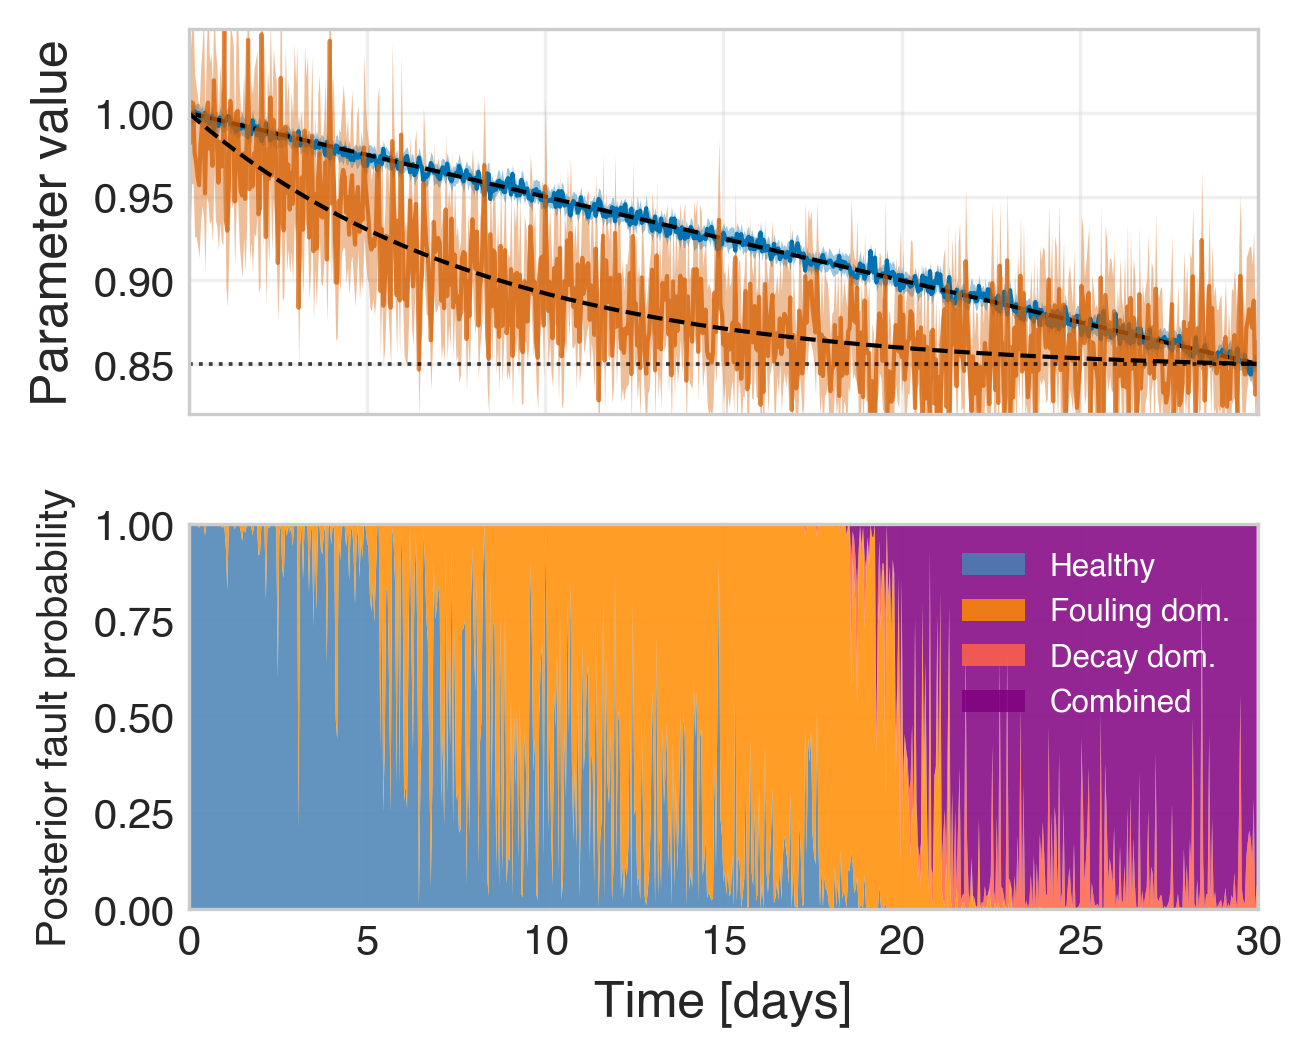
\includegraphics[width=0.97\linewidth]{10_degradation_tracking}
  \caption{30-day sequential degradation tracking for System~I (720 consecutive
    60-min windows, linear $\alpha$ decay and Kern--Seaton $\beta$ fouling).
    SBI posterior mean (solid) and 90\% CI (shaded) for
    $\alpha(t)$ (top row) and $\beta(t)$ 
    (bottom row) overlaid on the true degradation profile (dashed).
    The $\beta$ trace runs approximately $0.08$ below the true curve --- the
    structural closed-loop bias characterised in Section~\ref{sec:identifiability}
    --- while the 90\% CI correctly brackets the truth throughout.}
  \label{fig:tracking}
\end{figure}
% ------------------------------------------------------------------

% =============================================================
\section{Results: System~II --- Luyben Reactor-Column-Recycle Plant}
\label{sec:results_system2}
% =============================================================

%Results for System~II (Wu et al.~\citeyearpar{Wu2003}) are presented belowfollowing the same structure as Section~\ref{sec:results_system1}: summarystatistics, structural identifiability, fault classification, and degradation tracking.  
For System~II, the central finding is that all three apparent joint
non-identifiabilities uncovered by the 66-D summary-statistic representation are representation artefacts rather than properties of the plant, while the one genuine identifiability limitation, reactor temperature masking by Loop~1, transfers exactly from System~I.

\subsection{Physics-Informed Summary Statistics for System~II}
\label{sec:wu_summary_stats}
% ---------------------------------------------------------------------------

Similar to System I, each 2-hour observation window is compressed into
a 66-dimensional summary-statistic vector prior to passing it to the neural
density estimator. The complete feature definitions, per-parameter 
mutual-information rankings, and PCA-based separability analyses are detailed
in the Supporting Information.

Among these features, two physics-informed proxies carry the dominant identifying
information for the five degradation parameters. the System~II analogue of $s_{U\!A}$ for System~I (Eq.~\eqref{eq:ua_proxy}), is given by:

\begin{equation}
  s_{UA,r} = \frac{T_r - T_j}{Q_j} \propto (\beta_r\!\cdot\!U\!A_r)^{-1} \, .
  \label{eq:wu_ua_proxy}
\end{equation}
%
Under Loop~1 PI control,
$T_r \approx T_\mathrm{sp}$ and the numerator encodes the jacket temperature
drop driven by fouling, while the denominator normalises by the controller
output.  The normalised recycle flow deviation
%
\begin{equation}
  s_{F_R} = F_{R,\mathrm{norm}} - 1
  \label{eq:wu_fr_proxy}
\end{equation}
%
provides the primary snowball indicator. Any reduction in per-pass conversion (lower $\alpha$ or $\eta_\mathrm{col}$) drives $F_{R,\mathrm{norm}}$ above 1.
Because both parameters raise $s_{F_R}$ in the same direction, $s_{F_R}$ alone cannot distinguish catalyst decay from column-efficiency loss and a confound is to be expected. The identifiability analysis in Section~\ref{sec:wu_identifiability} investigates this directly.

\subsection{Fault Classification}
\label{sec:wu_fault_class}
% ---------------------------------------------------------------------------

Three candidate joint parameter confounds emerge under the 66-D
summary-statistic representation used for System~II, and all three
are shown in the identifiability analysis below
(Section~\ref{sec:wu_identifiability}) to be artefacts of that representation
rather than physical properties of the plant. For reference in what follows:
\emph{Artefact~1} is the $(\alpha,\eta_\mathrm{col})$ pair
(Section~\ref{sec:wu_artifact1}), \emph{Artefact~2} is $(\alpha,\beta_r)$
(Section~\ref{sec:wu_artifact2}), and \emph{Artefact~3} is the
$(\alpha/\beta_r, z_{A0,\mathrm{eff}})$ pair (Section~\ref{sec:wu_artifact3}).
Their consequences for the classification results differ sharply
depending on whether the confused parameters share a fault-taxonomy unit.

The calibrated posterior is applied to the 14 closed-loop fault
scenarios (30 stochastic replicates each, 200 posterior draws per replicate).
Unit-level classification uses the same posterior-mass approach as System~I
(Section~\ref{sec:fault_class}), with threshold $\theta_\mathrm{thr} = 0.85$
applied to each of the five degradation parameters. As established in 
Section~\ref{sec:fault_class}, classification is reported at the operationally 
relevant fault-unit level rather than the scenario level to ensure robust 
detection despite local parameter confounds.


% ------------------------------------------------------------------
\begin{table*}[thbp]
\centering
\caption{Unit-level fault classification results for System~II
  (14 scenarios, 30 replicates for each calibrated posterior,
  $\theta_\mathrm{thr}=0.85$). Per-class F\textsubscript{1} is the
  harmonic mean of precision and recall across all replicates in each fault-unit category.}
\label{tab:wu_classification}
\small
\begin{tabular}{llrl}
\toprule
Fault unit & Scenarios & $F_1$ & Note \\
\midrule
Healthy  & W1                  & 0.667 & Some healthy replicates border the threshold \\
Reactor  & W2--W6, W11, W15    & 0.948 & Near-perfect despite $(\alpha,\beta_r)$ corr = 0.998 \\
Column   & W7, W9              & 1.000 & $\eta_\mathrm{col}$ and $\xi_\mathrm{reb}$ well-identified \\
Feed     & W10                 & 0.000 & Artefact~3 confound with $\alpha$ (Section~\ref{sec:wu_artifact3}) \\
Multi    & W12, W13, W16       & 0.854 & W13 weak (7/30): feed+reactor compound, Artefact~3 \\
\midrule
\multicolumn{2}{l}{Overall macro-F1} & 0.694 & 87.4\% accuracy \\
\bottomrule
\end{tabular}
\end{table*}
% ------------------------------------------------------------------

% ------------------------------------------------------------------
\begin{figure}[htbp]
  \centering
  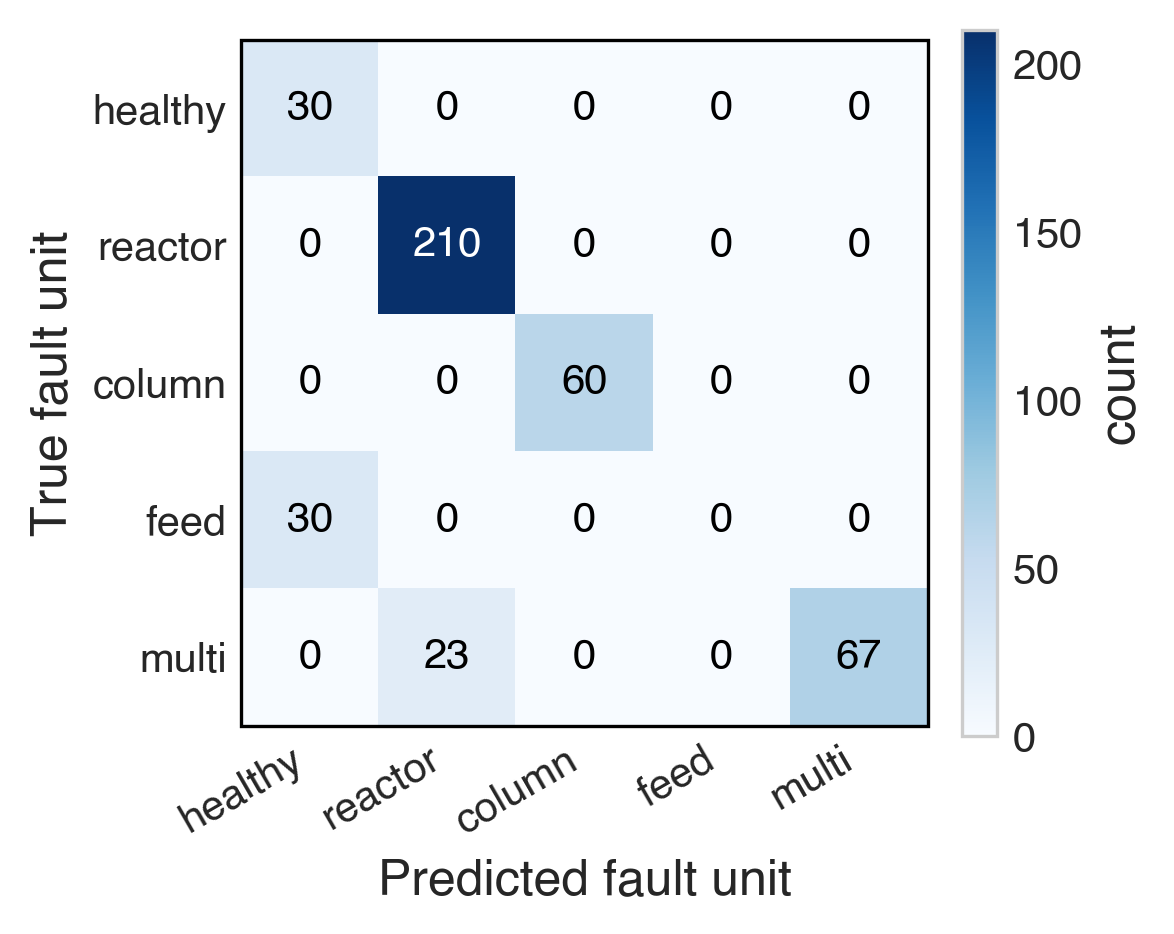
\includegraphics[width=0.9\linewidth]{nb31_confusion_matrix}
  \caption{Unit-level fault confusion matrix for System~II (14 scenarios,
    30 replicates each). Rows: true fault unit; columns: predicted fault unit.
    Reactor and column faults are reliably detected. Feed-fault scenarios
    (W10, W13) are predominantly misclassified as reactor or compound faults as a 
    the consequence of the representation-level $(\alpha, z_{A0,\mathrm{eff}})$
    confound identified in Section~\ref{sec:wu_artifact3}.}
  \label{fig:wu_confusion}
\end{figure}
% ------------------------------------------------------------------

Overall unit-level classification accuracy is 87.4\% with macro-F1~$= 0.694$. Per-unit results are summarised in Table~\ref{tab:wu_classification} and the
confusion matrix is shown in Figure~\ref{fig:wu_confusion}.

Breaking down the performance by functional unit reveals how representation 
artefacts impact downstream diagnosis:
\begin{itemize}
    \item \textit{Reactor faults succeed despite parameter-level confound:} 
    The reactor-fault scenarios (W2--W6, W11, W15) are classified correctly
    in 30/30 replicates, despite the strong $(\alpha, \beta_r)$ confound.
    Because both parameters trigger the same reactor-unit alarm, the confound 
    corrupts parameter-level attribution (which of $\alpha$ or $\beta_r$ is degraded) 
    but leaves unit-level detection intact.
    
    \item \textit{Column faults and the Artefact 1 retraction:} 
    Scenario W12 ($\alpha=0.75$, $\eta_\mathrm{col}=0.80$) classifies correctly as
    a compound fault in 30/30 replicates with zero leakage. This directly
    confirms the retraction of the $(\alpha, \eta_\mathrm{col})$ banana claim
    (Artefact~1, Section~\ref{sec:wu_artifact1}): under the full feature set,
    the two parameters are already sufficiently resolved for reliable unit-level
    attribution without requiring a composition analyser.
    
    \item \textit{Feed faults fail completely:} 
    The feed-purity scenario W10 achieves $F_1 = 0.000$. All 30 replicates are
    misclassified as reactor or compound faults, a direct consequence of the
    Artefact~3 $(\alpha, z_{A0,\mathrm{eff}})$ confound under the 66-D summary-statistic
    representation (Section~\ref{sec:wu_artifact3}). Because this confound bridges 
    two entirely distinct physical units, it fatally disrupts detection.
\end{itemize}

%\paragraph{\textbf{Comparison against the Extended Kalman Filter (EKF).}}
Table~\ref{tab:wu_ekf_classification} places the SBI classification alongside 
the baseline EKF estimates. The EKF structurally cannot observe $z_{A0,\mathrm{eff}}$ 
(estimating only $[\alpha,\beta_r,\eta_\mathrm{col}]$), offering no comparison point at W10. 
Where the EKF does produce estimates, two distinct regimes emerge. At the 
near-snowball scenarios W12 and W15 ($\alpha = 0.75$ and $\alpha = 0.58$ respectively), 
the EKF achieves only 3\% empirical coverage on $\alpha$, reflecting a genuine, 
representation-independent failure of Gaussian linearisation under strong nonlinear 
recycle dynamics near the tipping point. SBI, conversely, achieves 100\% coverage at W15. 
At W11, the EKF's 0\% coverage is a tuning-sensitive pitfall rather than evidence 
of a genuine degeneracy, as an independently re-tuned EKF with raw-trajectory 
access recovers both parameters to $<2$\% error (Section~\ref{sec:wu_artifact2}). 
Crucially, SBI's unit-level classification remains correct across all three of these 
scenarios (W11, W12, W15) regardless of baseline tuning sensitivities.

% ------------------------------------------------------------------
\begin{table*}[htbp]
\centering
\caption{SBI vs.\ EKF at the scenarios used to illustrate fault-classification
  robustness (System~II). The augmented EKF
  (Section~\ref{sec:wu_sequential}) estimates only $[\alpha,\beta_r,\eta_\mathrm{col}]$ whereas
  $\xi_\mathrm{reb}$ and $z_{A0,\mathrm{eff}}$ are outside its augmented state and are therefore unobservable to it by construction, not merely difficult to estimate.}
\label{tab:wu_ekf_classification}
\small
\begin{tabular}{llllll}
\toprule
Scenario & True fault unit & SBI classification           & EKF estimate & EKF 90\% coverage & Note \\
\midrule
W10 & Feed ($z_{A0,\mathrm{eff}}=0.75$)  & Misclassified,  & --- & --- & $z_{A0,\mathrm{eff}}$ not in EKF's  \\
    &                                    & $F_1=0.000$ &  & & augmented state \\

W11 & Reactor ($\alpha=\beta_r=0.80$)    & Correct, 30/30 & $\hat\alpha=0.907$,& 0\% & Tuning-sensitive; see Artefact~2 \\
       &                                     & & $\hat\beta_r=0.986$ &  & \\
W12 & Multi ($\alpha=0.75$)              & Correct, 30/30 & $\hat\alpha\approx1.19$ & 3\% & Snowball nonlinearity \\
W15 & Reactor ($\alpha=0.58$)            & Correct, 30/30 & $\hat\alpha=0.990$ & 3\% & Near snowball tipping point \\
\bottomrule
\end{tabular}
\end{table*}
% ------------------------------------------------------------------



% ---------------------------------------------------------------------------
\subsection{Structural Identifiability Analysis}
\label{sec:wu_identifiability}
% ---------------------------------------------------------------------------


% ------------------------------------------------------------------
\begin{figure}[tbp]
  \centering
  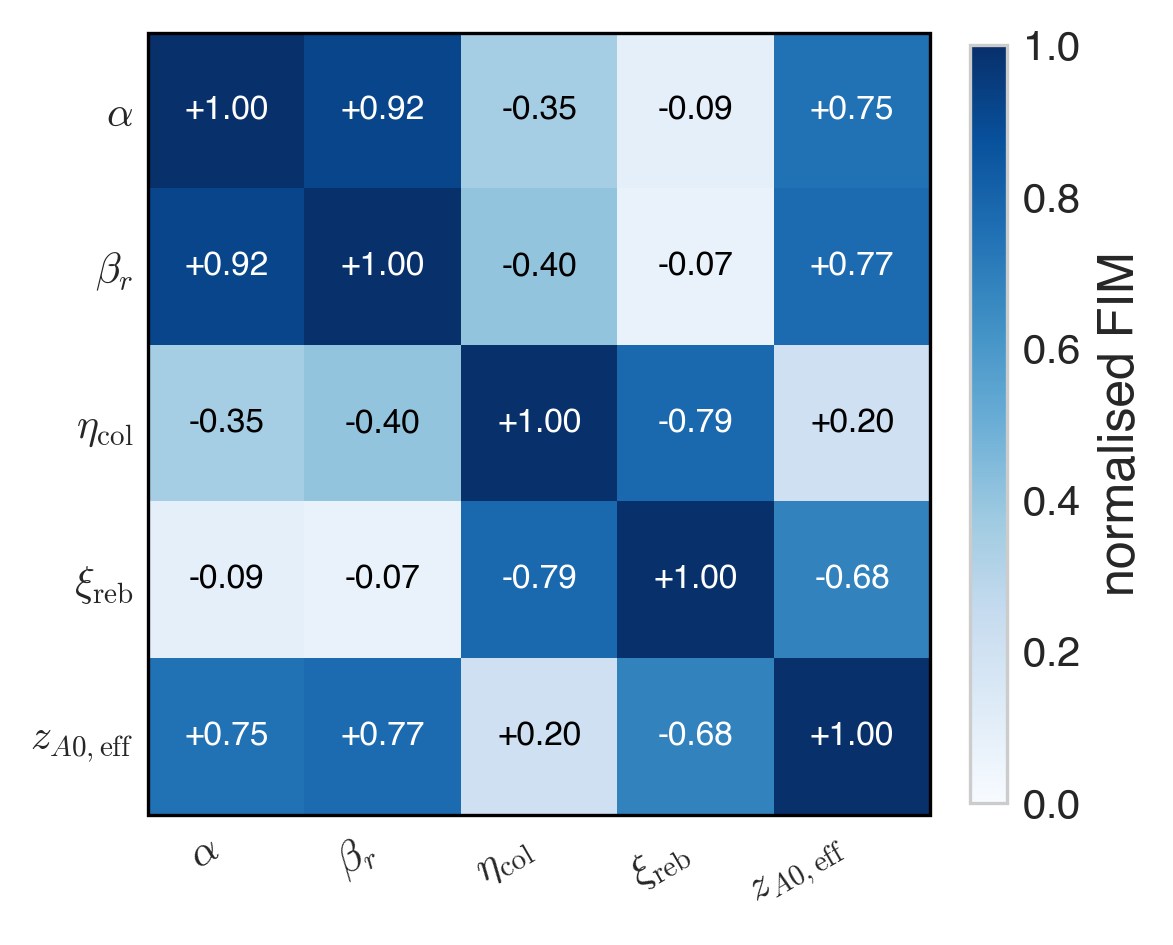
\includegraphics[width=0.97\linewidth]{nb23_fim_heatmap_single}
  \caption{Normalised $5\times5$ Fisher information 
  matrix at System II nominal
    operating point.
    Entries show the signed, normalised parameter coupling at the nominal operating point, with colour intensity indicating absolute information coupling strength. The strong positive $\alpha-\beta_r$
  off-diagonal term highlights a dominant identifiability confounding between reactor degradation and reactor heat-transfer loss, while the remaining structure shows weaker or more localized couplings among column efficiency, reboiler efficiency, and feed composition.
  The high off-diagonal $+0.93$ for $(\alpha,\beta_r)$
    under the full feature set is investigated as a potential joint degeneracy in
    Sections~\ref{sec:wu_artifact1}--\ref{sec:wu_artifact3}.}
  \label{fig:wu_fim}
\end{figure}
% ------------------------------------------------------------------


Similar to System~I, System~II raises the question of which apparent
identifiability limits are genuine, representation-independent properties of
the closed-loop plant, and which are artefacts of the 66-D summary-statistic
representation used to train the posterior? 
%The scalar masking mechanism discussed immediately below
%is genuine and representation-independent; the three joint (two-parameter)
%confounds 
%discussed in Sections~\ref{sec:wu_artifact1}--\ref{sec:wu_artifact3}
%are all shown to be representation artefacts, not properties of the plant ---
%with, as Section~\ref{sec:wu_fault_class} demonstrates, materially different
%consequences for downstream fault classification depending on which unit the
%confused parameters belong to.

The Fisher Information Matrix (FIM) analysis is performed on the 66-D summary-statistic representation
at the nominal (healthy) operating point ($\alpha = \beta_r = \eta_\mathrm{col}
= \xi_\mathrm{reb} = 1.0$, $z_{A0,\mathrm{eff}} = 0.90$). The resulting normalised $5\times5$ FIM at the nominal operating point is shown in Figure~\ref{fig:wu_fim}. The identifiability
structure of System~II differs qualitatively from System~I in two respects.
First, the scalar masking mechanism that makes $\beta$ hard to identify in
System~I (Section~\ref{sec:identifiability}) transfers exactly to both
$\alpha$ and $\beta_r$ here, because Loop~1 holds $T_r = T_\mathrm{sp}$
regardless of which thermal fault is present:
$\partial T_{r,\mathrm{ss}}/\partial\alpha \equiv \partial T_{r,\mathrm{ss}}/\partial\beta_r \equiv 0$.
However, the ratio $I_{\alpha\alpha}/I_{\beta_r\beta_r} \approx 1.1$--$1.4\times$
across operating points is milder than System~I's 250--500$\times$ because
System~II has no observable concentration channel to give $\alpha$ a privileged
primary observable. Both parameters are restricted to the same noisier
secondary channels ($T_j$, $Q_j$, $F_{R,\mathrm{norm}}$), making their scalar
information deficits roughly symmetric. They both remain identifiable, but with a
mild, shared precision penalty relative to a system with an independent
primary channel for $\alpha$.

Second, and more significantly, the 66-D summary-statistic representation
generates three apparent joint (two-parameter) confounds that do not survive
a representation-level check.  
Each of the three candidates is examined with the same procedure, which
we refer to as the \emph{raw-trajectory Fisher-information (RT-FIM) check}. A
joint degeneracy surfaced by a compressed-feature Fisher-information or SBI
analysis in a closed-loop system is treated as provisional until it survives a
comparison against the raw, unaggregated trajectory of the same observed
channels. The check requires only the simulator already used to train the
posterior, not additional instrumentation. We first compute the FIM on the
production whole-window summary statistics and record the normalised
off-diagonal for the candidate pair, then recompute the identical FIM on the
raw trajectory at the same operating point(s), using matched noise seeds. The
two representations are compared not only through their normalised
off-diagonals, but also through their Cram\'er-Rao standard deviations and
condition numbers (Section~\ref{sec:identifiability}). A genuine resolution of
the pair must improve the conditioning, not merely shrink one off-diagonal
entry.

We also include a negative control at a modestly finer time resolution, but still
whole-window-style, such as sub-window mean and spread
statistics. This rules out a cheap feature-engineering fix before concluding
that only the raw trajectory resolves the pair. The cost is small relative to
the training budget it protects. At the replicate count used throughout this
paper ($n=60$ replicates to estimate $\boldsymbol{\Sigma}$, plus two evaluations
per parameter for the central-difference Jacobian), one representation at one
operating point costs on the order of 70 simulator calls, several orders of
magnitude cheaper than the 10,000--20,000 simulations used to train the
production posterior itself.

As a check on the diagnostic's specificity, we additionally applied the
RT-FIM check to a parameter pair with no plausible physical coupling
$(\beta_r,\xi_\mathrm{reb})$. They belong to different physical units (reactor jacket
versus reboiler), different control loops, and with no shared mechanism. The
normalised off-diagonal is small under both the summary-statistic and
raw-trajectory representations, at both the nominal operating point and a
$\xi_\mathrm{reb}$-faulted scenario, confirming that the 66-D representation
does not manufacture spurious coupling indiscriminately. The three
retractions below are a property of the specific parameter pairs
identified, not an artefact of the check itself.

\subsubsection{Artefact 1: Restricted-channel confound between
  \texorpdfstring{$\alpha$}{alpha} and
  \texorpdfstring{$\eta_\mathrm{col}$}{eta_col}}
\label{sec:wu_artifact1}

Both catalyst decay and column-efficiency loss increase the A reactant fraction leaving
the reactor and therefore raise the recycle flow $F_{R,\mathrm{norm}}$ via the
snowball mechanism ("column" Scenario W12).  When the identifiability scan is restricted to
$F_R$-derived summary features, the two parameters produce an extended
degenerate ridge with the classic banana shape.  However, combining $F_R$ with
the column's own reboiler channels ($T_\mathrm{reb}$, $Q_\mathrm{reb}$),
both already part of the standard measurement set, substantially resolves
the ridge. The two channels' individual ambiguities run at different angles in
$(\alpha, \eta_\mathrm{col})$ space, and their intersection is a compact region
near the true value.  The calibrated posterior corroborates this: the
$\eta_\mathrm{col}$ 90\% credible-interval width is $\approx 0.01$--$0.02$
across tested scenarios, with $|\mathrm{corr}(\alpha, \eta_\mathrm{col})| < 0.15$.
This apparent confound is therefore a restricted-channel artefact, not a
property of the plant.

\subsubsection{Artefact 2: Temporal-aggregation confound between
  \texorpdfstring{$\alpha$}{alpha} and
  \texorpdfstring{$\beta_r$}{beta_r}}
\label{sec:wu_artifact2}

The $(\alpha, \beta_r$ in "reactor" Scenario W11) pair presents a deeper challenge: the Fisher-information
off-diagonal reaches $+0.901$ at nominal operation under the 66-D feature set, and
this coupling \emph{survives combination of the entire 66-D feature vector}. It cannot be eliminated by adding more whole-window statistics of the same kind. At the compound-fault scenario W11 ($\alpha = 0.80$, $\beta_r = 0.80$),
the trained, calibrated posterior yields $\mathrm{corr}(\alpha,\beta_r) = +0.998$,
consistent with the FIM finding.

To determine whether this coupling is physical or representational, we applied
the same FIM methodology to the \emph{raw, unaggregated} trajectory of the
three already-observed channels ($T_r$, $T_j$, $F_{R,\mathrm{norm}}$), computing
$\mathbf{I} = \mathbf{J}^\mathsf{T}\boldsymbol{\Sigma}^{-1}\mathbf{J}$ on the
full 120-step time series rather than on their whole-window summary statistics.
The off-diagonal collapses from $+0.85$--$+0.90$ to $\approx 0.00$,
reproducibly across noise seeds and at multiple operating points. A negative
control using sub-window statistics at $6\times$ finer time resolution (108-D)
shows \emph{no} improvement ($+0.60$--$+0.86$), confirming that the missing
information is encoded in fine-grained transient shape, not in coarser level
or spread statistics. An independently re-tuned EKF with raw-trajectory access
corroborates this, recovering $\alpha$ and $\beta_r$ to $<2$\% error at the same
operating points that the summary-statistic FIM classifies as non-identifiable.
As Section~\ref{sec:identifiability} argues, a shrinking off-diagonal alone
does not rule out that the ellipse merely changed angle without shrinking in
size; the condition number of $\mathbf{I}$ answers that directly. At W11 it
falls from $3.45\times10^3$ under the 66-D representation characterising an
almost-degenerate ridge, consistent with the $+0.90$ off-diagonal, to
$5.34$ under the raw trajectory, indicating a well-conditioned, near-round region.  This
$\sim\!650\times$ improvement in conditioning is independent confirmation
that the achievable precision genuinely improved, rather than the
off-diagonal being diluted by the extra dimensions of the raw representation.
The $(\alpha, \beta_r)$ coupling is therefore a lossy temporal-aggregation
artefact of the 66-D representation, not a physical property of the plant.

Which specific features carry this coupling clarifies when practitioners
should expect the problem to recur, rather than leaving ``whole-window
aggregation is lossy'' as an empirical tally. Decomposing the off-diagonal
feature by feature shows that the mean and representative quantile
of the whole-window jacket cooling duty $Q_j$ together account for $\approx65$--$70\%$ of the
total coupling at W11 (and more at the nominal point), robust across noise
seeds. This is not a coincidence: both $\alpha$ and $\beta_r$ act on the
reactor energy balance that Loop~1 compensates for by adjusting $Q_j$, and to
first order a less active catalyst (less heat generated) and a more fouled
jacket (less heat removed) both require a similar shift in the
\emph{steady-state level} of $Q_j$ to hold $T_r$ at setpoint. A whole-window
mean or quantile of $Q_j$ cannot distinguish the two mechanisms as this requires the
fine-grained \emph{transient} shape of the $Q_j$ trajectory (how quickly
and in what pattern it approaches its new level),
which is exactly the information a whole-window statistic discards and the
raw trajectory retains. Formally, whole-window aggregation is a linear map
$\mathbf{A}$ from the raw trajectory to the summary vector, so
$\mathbf{J}_\mathrm{summary} = \mathbf{A}\,\mathbf{J}_\mathrm{raw}$. A
low-rank $\mathbf{A}$ can align two parameters' otherwise-distinguishable
sensitivity directions purely as an artefact of the projection, independently
of how informative the raw signal actually is.  The mechanism therefore
generalises beyond the two parameters studied here. It should recur whenever
two fault parameters act through a shared actuator or controlled variable and
are compressed to the same coarse, whole-window statistics of that channel.

Despite this confound, Section~\ref{sec:wu_fault_class} shows unit-level fault
classification at W11 is correct in 30/30 replicates. Because $\alpha$ and
$\beta_r$ map to the \emph{same} reactor fault unit, the confound corrupts
parameter-level attribution without
corrupting unit-level detection that a reactor fault is present at all.

\subsubsection{Artefact 3: Composition-confound between reactor faults and feed
  purity}
\label{sec:wu_artifact3}

A third representation artefact was identified through the fault-classification
analysis (Section~\ref{sec:wu_fault_class}): the feed-purity parameter
$z_{A0,\mathrm{eff}}$ ('feed' Scenarios W10 and W13) shows a near-degeneracy with both $\alpha$ and $\beta_r$
under the 66-D feature set at degraded operating points (FIM off-diagonal
$\approx -0.89$ at the W2-truth, compared to $\approx -0.12$ at nominal).
Applying the raw-trajectory FIM test again collapses this off-diagonal to
$\approx -0.07$, the same signature as Artefact~2.  As with Artefact~2, the
condition number of $\mathbf{I}$ confirms this is a genuine tightening of the
achievable precision rather than a diluted correlation. At the W2-truth it
falls from $4.36\times10^3$ under the 66-D representation to $5.48$ under the
raw trajectory, and at the W5-truth (the analogous $(\beta_r,z_{A0,\mathrm{eff}})$
coupling) from $41.4$ to $5.24$.  Both faults shift
overlapping recycle- and conversion-related features in similar directions such that
the summary-statistic compression conflates ``a reactor fault is present''
with ``feed purity has drifted.'' This is the third independent instance of
the same mechanism where every apparent joint non-identifiability surfaced by the
66-D whole-window representation and subsequently tested against a raw-trajectory
FIM has collapsed to near-zero, consistent with the representation being the
source of the confound rather than the plant physics.

Unlike Artefact~2, this confound's downstream consequence is severe rather
than benign as Section~\ref{sec:wu_fault_class} shows it drives feed-fault
classification to $F_1 = 0.000$ (scenario W10) and drags down the
compound-fault $F_1$ at W13. The reason is exactly the mirror image of
Artefact~2's benign case where $z_{A0,\mathrm{eff}}$ maps to its \emph{own}, distinct
feed fault unit rather than sharing a unit with $\alpha$ or $\beta_r$, so this
representation artefact corrupts unit-level detection directly, not merely
parameter-level attribution within an already-correctly-detected unit.
Whether a joint representation confound is classification-benign or
classification-severe therefore depends on the fault taxonomy, not just on
the confound's Fisher-information magnitude. Artefact~2 and Artefact~3 have
comparable off-diagonal strength under the 66-D representation, yet only the
latter breaks fault detection.



%\textit{CNN embedding on raw trajectories.}
To test whether a neural embedding trained directly on raw $120\times9$ 
time series could bypass the representation artefacts identified in
Sections~\ref{sec:wu_artifact1}--\ref{sec:wu_artifact3}, a CNN-based SBI
posterior (62,686-parameter CNN, 30-dimensional learned embedding was trained on
$n_\mathrm{sim}=15{,}000$ raw trajectories with the same NSF
architecture as the hand-crafted posterior. 
%Training is seed-unstable at the
%same order of difficulty as the hand-crafted pipeline (Section~S9.2): only 1
%of 8 seeds passed simulation-based calibration, underscoring that marginal SBC
%alone does not certify that a specific joint-posterior shape has been learned
%correctly.

The three artefacts respond differently to the richer representation.
\emph{Artefact~1} ($\alpha,\eta_\mathrm{col}$, W12) remains resolved under the
CNN, exactly as under the hand-crafted posterior (correlation $+0.010$ vs.\
$+0.011$) providing an independent corroboration of the restricted-channel diagnosis
(Section~\ref{sec:wu_artifact1}) using an entirely different representation.
\emph{Artefact~2} ($\alpha,\beta_r$, W11) does \emph{not} narrow: the
joint-posterior correlation is $+0.993$ under the CNN versus $+0.998$ under
the hand-crafted posterior, essentially unchanged, and this null result is
robust across 19 tested (seed, operating-point) combinations, not a
single-point artefact. \emph{Artefact~3} ($\alpha, z_{A0,\mathrm{eff}}$,
W10/W13) \emph{does} collapse under the CNN, from $\approx+0.99$
(hand-crafted) to $\approx-0.004$ (CNN) providing a second, non-linearised
confirmation of the raw-trajectory FIM diagnosis for this pair
(Section~\ref{sec:wu_artifact3}).

This split distinguishes \emph{information-theoretic} recoverability ---
established for all three artefacts by the FIM, %and for Artefact~2
%additionally by a re-tuned EKF with raw-trajectory access
%(Section~\ref{sec:wu_artifact2}) --- 
from recoverability \emph{by this
specific trained estimator at a modest training budget}, which succeeds for
Artefacts~1 and~3 but not Artefact~2.

Despite resolving Artefact~3's correlation, the CNN posterior does
\emph{not} improve feed-fault classification where $F_1=0.000$ for the feed class
under both representations (Supporting Information Table~S10.3), and W10 still
misclassified in all 30 replicates, but for a different reason under each
representation. Under the hand-crafted posterior, the
$(\alpha,z_{A0,\mathrm{eff}})$ correlation itself pulls posterior mass toward
\emph{healthy}. Under the CNN, that correlation is gone, but the posterior
carries its own systematic downward bias in $\alpha$ which is present across
essentially all scenarios, including the healthy baseline pushing
W10 samples across the reactor threshold.  This same $\alpha$ bias
degrades overall classification such macro-F1 falls from 0.694 to 0.270 and the
accuracy from 87.4\% to 61.9\% (Supporting Information Table~S10.3).
%Sequential tracking is similarly mixed (Section~\ref{sec:wu_sequential}): the
%CNN improves $\beta_r$ tracking (MAE $0.198\rightarrow0.139$) but worsens
%$\alpha$ tracking ($0.048\rightarrow0.067$), both still far short of the EKF.


\subsection{30-Day Sequential Degradation Tracking}
\label{sec:wu_sequential}
\begin{figure}[t]
    \centering
    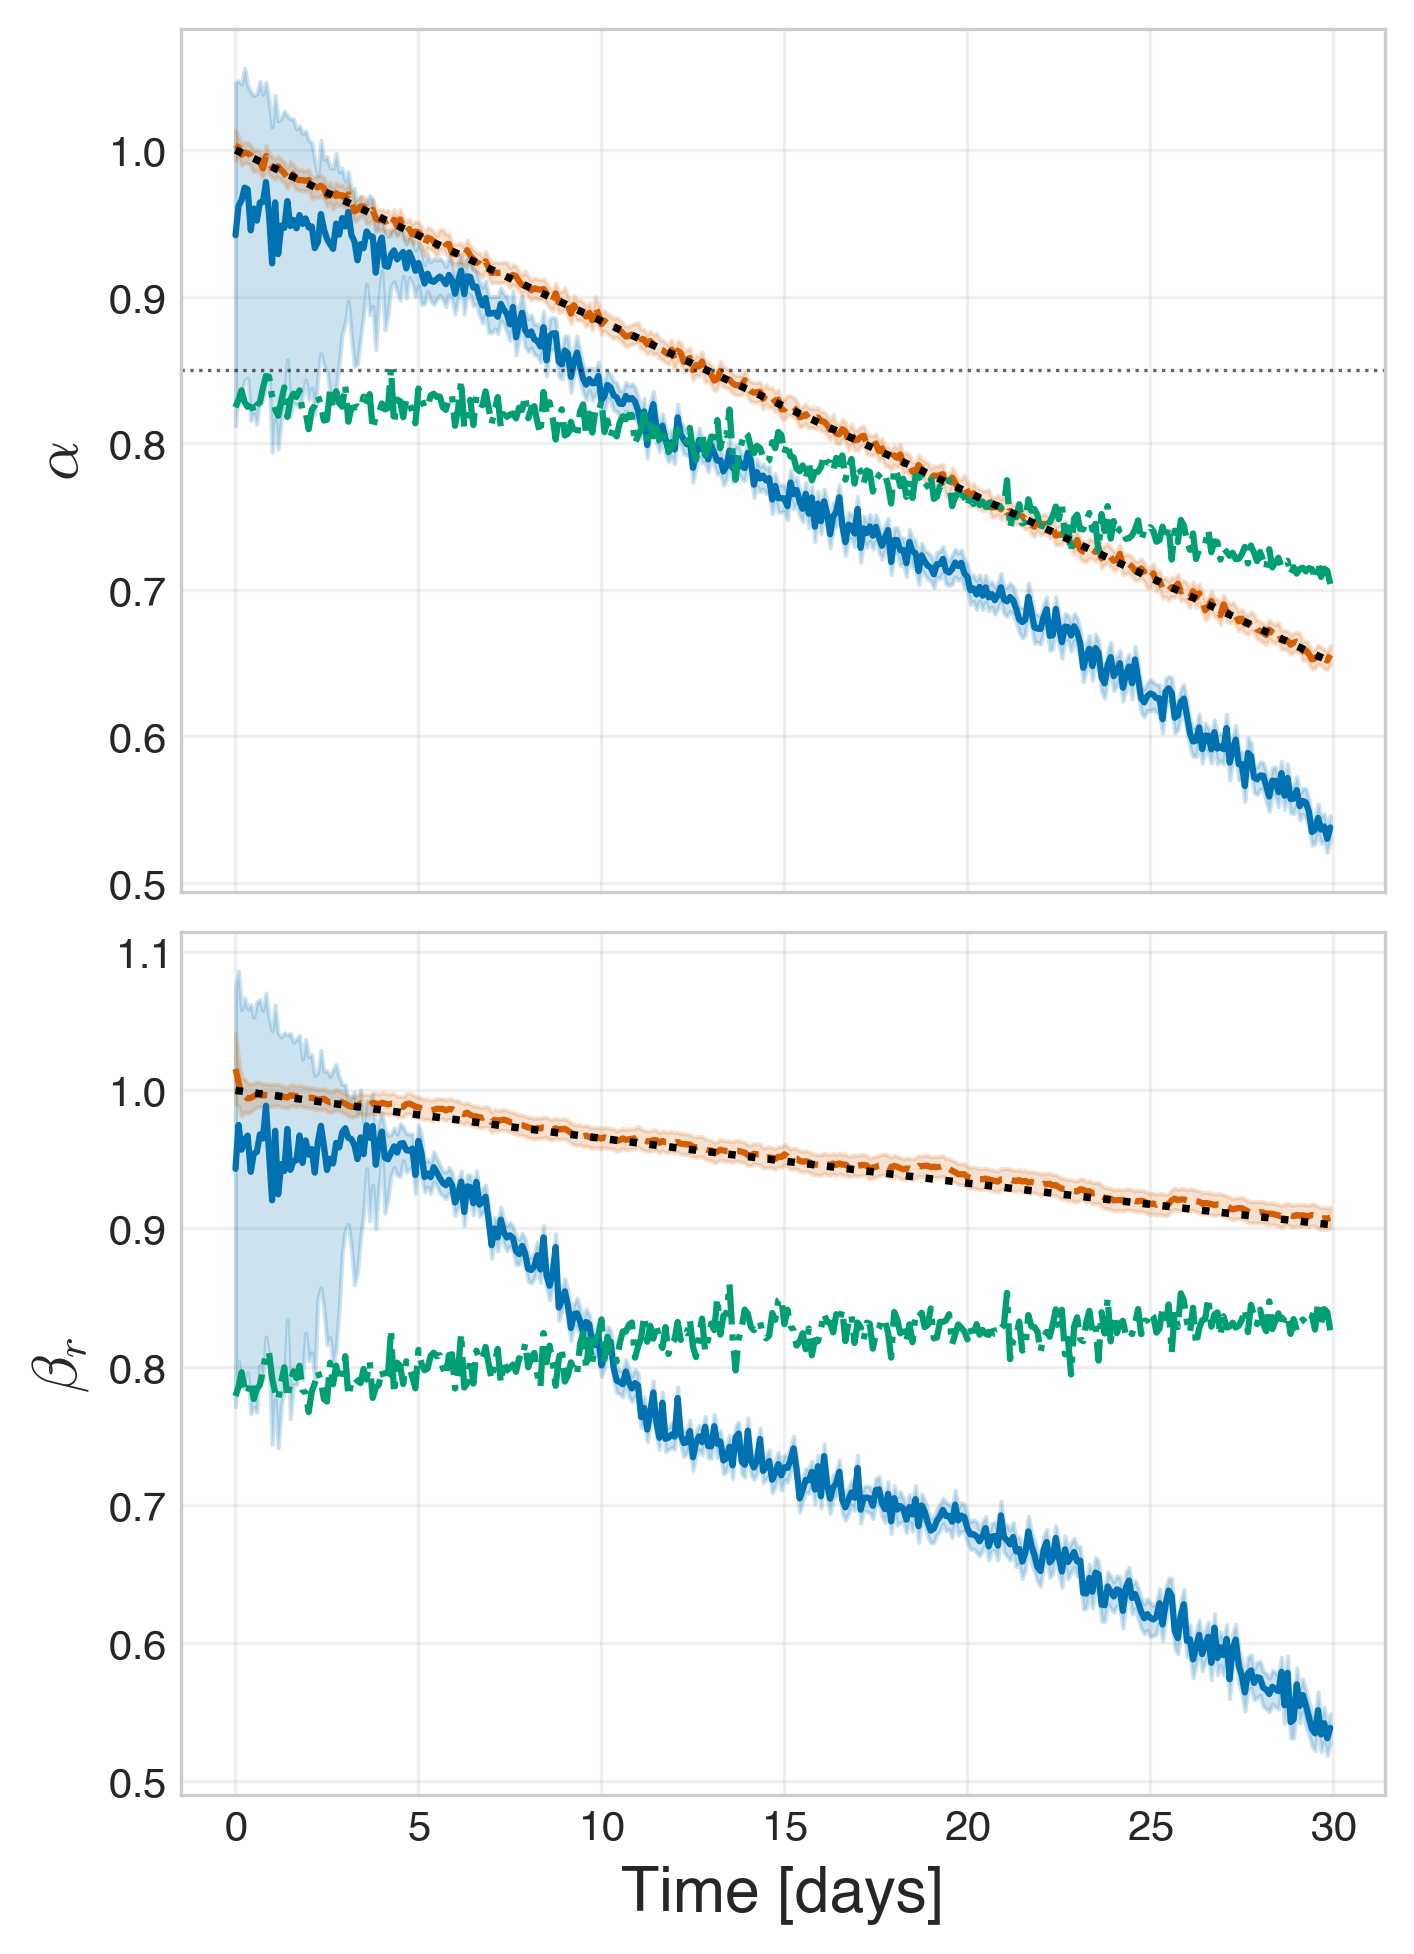
\includegraphics[width=0.95\linewidth]{nb27_sequential_tracking.png}
    \caption{Sequential System II degradation tracking over 30 days. The true trajectories for catalyst activity 
    $\alpha$ $\beta_r$ and reactor heat-transfer factor 
  are compared with independent amortised SBI estimates (blue), recursive EKF estimates (orange), and CNN-embedding SBI posterior means (green) across 360 two-hour windows. Shaded bands show 90$\%$ intervals for SBI and EKF only. The EKF tracks both slowly varying parameters closely, while the amortised SBI methods show larger bias and delayed response, especially for $\beta_r$, illustrating the difficulty of recovering gradual degradation from independent window-level posterior inference.}
    \label{fig:sysII_track}
\end{figure}

The calibrated  posterior is applied to a synthetic 30-day
monitoring stream of 360 consecutive 2-hour observation windows, each
processed independently (no temporal state carried between windows). The
degradation profile follows a linear catalyst decay reaching $\alpha \approx
0.65$ and a Kern--Seaton fouling curve reaching $\beta_r \approx 0.90$ by day
30, with $\eta_\mathrm{col}$, $\xi_\mathrm{reb}$, and $z_{A0,\mathrm{eff}}$
held at their healthy values throughout. Results are shown in 
Figure~\ref{fig:sysII_track}.

Unlike every other SBI-vs-EKF comparison, the EKF outperforms
SBI here with $\mathrm{MAE}_\alpha = 0.048$ (SBI) vs.\ $0.002$ (EKF), and
$\mathrm{MAE}_{\beta_r} = 0.198$ (SBI) vs.\ $0.004$ (EKF). This is not evidence
that SBI cannot exploit sequential structure, nor that $(\alpha,\beta_r)$ is
genuinely non-identifiable. Control experiments (Supporting
Information~\S{}S11) rule out any advantage from accumulating information
across the 360-window run, and instead trace the gap to the EKF's privileged
access to the raw, unaggregated trajectory through the exact ODE model
consistent with Artefact~2 (Section~\ref{sec:wu_artifact2}). The CNN-embedding
posterior (Supporting Information Section~S10) narrows part of this gap
($\mathrm{MAE}_{\beta_r}$ improves to $0.139$) but not all of it
($\mathrm{MAE}_\alpha$ worsens to $0.067$), both still an order of magnitude
short of the EKF. SBI remains substantially faster per window (15~ms vs.\
25.9~ms for the EKF). %Full control experiments, the tracking figure, and per-window metrics are given in Supporting Information~\S{}S11.
% Full CNN results --- SBC calibration, per-scenario correlations, and 30-day
%tracking --- are given in Supporting Information Section~S10.


% ===========================================================================
\section{Discussion}
\label{sec:discussion}
% ===========================================================================

\subsection{One Genuine Limit, Three Representation Artefacts}
\label{sec:disc_limit_artefacts}

Both systems share one genuine, representation-independent identifiability
limit namely a high-gain feedback loop which drives
$\partial(\text{controlled variable})/\partial\theta \equiv 0$ for a specific
parameter, eliminating its primary observable channel. For System~I this is
the $\beta$-on-$T$ masking (Section~\ref{sec:identifiability}, 250--500$\times$
Fisher-information deficit). The CNN-embedding posterior trained on raw
trajectories rules reproduces the same $-0.08$ bias to within 1\% and thereby rules out that the masking is an artifact of the 
hand-crafted 29-D summary statistics. 
For System~II the identical mechanism (Loop~1 holding $T_r = T_\mathrm{sp}$)
masks \emph{both} $\alpha$ and $\beta_r$ simultaneously, but far more mildly
(1.1--1.4$\times$), because System~II gives neither parameter an independent
concentration channel to fall back on.

Beyond this genuine limit, System~II's 66-D summary-statistic representation
surfaced three candidate \emph{joint} confounds, 
$(\alpha,\eta_\mathrm{col})$, $(\alpha,\beta_r)$, and
$(\alpha,z_{A0,\mathrm{eff}})$, each with a substantial Fisher-information
off-diagonal. Applying the same raw-trajectory FIM test used to certify
System~I's scalar bias as genuine retracted all three
(Sections~\ref{sec:wu_artifact1}--\ref{sec:wu_artifact3}) by collapsing every off-diagonal
to near zero once whole-window aggregation is removed. 
Therefore, a joint degeneracy surfaced by a
compressed-feature SBI or FIM analysis should be treated as provisional
until checked against a minimally-aggregated representation. 

The raw-trajectory FIM establishes \emph{information-theoretic} recoverability for all three artifacts. However, this is not identical to practical recoverability \emph{by a specific amortised estimator under a given training budget}. This is demonstrated for Artefact~2 for which the analogous CNN test could not resolve the parameters despite the raw-trajectory FIM indicating \emph{information-theoretic} recoverability (Section~\ref{sec:wu_artifact2}). 
New instrumentation remains necessary only for the genuine scalar masking, where
no summary statistic computable from the existing sensors can close the gap.

\subsection{Why Amortised SBI Is the Appropriate Instrument for This Problem Class}
\label{sec:disc_why_sbi}

%This section sets out why amortised SBI is well matched to closed-loop, multi-unit fault diagnosis as a problem class. The argument here is independent of any single scenario-by-scenario comparison with a specific alternative estimator; the EKF comparisons that follow next examine one such comparison in detail, but the case for SBI made here does not depend on its outcome. 
Five properties of SBI, each tied to a specific
demand of the closed-loop problem class, motivate its use for multi-unit fault diagnosis.

First, the closed-loop, multi-unit systems studied here have no tractable
likelihood. The three decentralised PI loops, actuator saturation, and
nonlinear recycle dynamics (the snowball effect) make an explicit noise
model over the summary-statistic vector intractable to derive in closed
form. Instead SBI requires a stochastic simulator which is already standard practice in process systems engineering as a validated mechanistic process model built and maintained for design,
control-loop tuning, and operator training long before any fault-diagnosis
application is considered. Simulation-based inference turns this
pre-existing asset directly into a Bayesian estimator, without requiring a
new likelihood derivation, a linearisation, or a closed-form noise
assumption for every fault scenario of interest.

Second, the resulting posterior geometry is not merely non-Gaussian as an
incidental technical detail, it is diagnostically informative in its own
right. Decentralised feedback control couples fault parameters through the
variables it regulates, and the shape of that coupling (tight cluster vs ridge) is part of the
diagnosis. ``We cannot distinguish which of two reactor-side parameters has
degraded, but we are confident a reactor fault is present'' is a
materially different, and more honest, statement than a point estimate
carrying an implied precision the data do not support. A flexible density
estimator represents this shape because the closed-loop plant produces it,
and doing so is a requirement of the problem, not a stylistic preference.

Third, because the posterior is estimated jointly over the full
five-parameter fault vector, it captures cross-unit dependency structure
that individual parameter diagnosis cannot represent.
Our taxonomy-dependence finding include two representation
artefacts of comparable Fisher-information strength (Artefact~2 and
Artefact~3) with opposite consequences for fault classification, depending
only on whether the confused parameters share a fault-taxonomy unit
(Section~\ref{sec:wu_fault_class}). These are visible only because the method
returns a full joint distribution over all five parameters simultaneously,
not five independent marginal estimates. Root-cause attribution in a
multi-unit plant is inherently a question about the joint structure of
possible faults, not about any one parameter in isolation.

Fourth, condition monitoring is not a one-off inference problem but performed on every observation window for the entire remaining life of the equipment. Amortised inference pays its computational cost once, at
training time, in exchange for a sub-20~ms posterior on every subsequent
window (Section~\ref{sec:sequential_tracking}).% --- the natural shape of a
%solution to a repeated, indefinite-horizon monitoring task, dictated by the
%operational pattern of plant-wide condition monitoring itself.

Fifth, deriving fault classification from posterior probability mass
against physically defined thresholds (Section~\ref{sec:fault_class})
requires no historical labelled-fault data. No plant operator maintains a
labelled archive of ``this trajectory was a catalyst-decay event'' recorded
under normal operating conditions. Faults are rare, costly to induce
experimentally, and often confounded with unrelated disturbances. The
prior and the simulator supply everything the method needs, in place of
data that closed-loop plants essentially never have.

Together, these five properties are why amortised SBI is the appropriate
instrument for closed-loop, multi-unit fault diagnosis of this kind,
independently of any single scenario-by-scenario comparison.%; the EKF
%regimes discussed next examine one such comparison in detail.

\subsection{Artefact Severity Depends on the Fault Taxonomy, Not Confound Magnitude}
\label{sec:disc_taxonomy}

Retracting a confound as non-physical does not mean it is harmless.
Artefact~2 and Artefact~3 have
comparable Fisher-information off-diagonals ($+0.90$ and $-0.89$) and are
retracted by the identical test, yet their consequence for fault
classification is opposite. Artefact~2 is classification-\emph{benign}:
unit-level detection at scenario W11 is correct
(Section~\ref{sec:wu_fault_class}) despite a high posterior correlation
because $\alpha$ and $\beta_r$ share the \emph{same} reactor fault
unit such that the confound corrupts only which of the two is attributed the
fault, not whether a reactor fault is detected. Artefact~3 is
classification-\emph{severe} as it drives feed-fault $F_1$ to $0.000$, because
$z_{A0,\mathrm{eff}}$ defines its \emph{own}, distinct fault unit, so an
equally-strong confound misattributes the unit entirely, not merely the
parameter. Whether a joint representation artefact
is classification-benign or classification-severe therefore depends on where
the confused parameters sit in the fault taxonomy, not on the raw magnitude
of the confound. This distinction is invisible to identifiability analysis
alone, and checkable only against the specific downstream decision the posterior
is used to make, and the reason fault classification is reported at the
fault-unit level (Section~\ref{sec:wu_fault_class}).

\subsection{EKF Failure and Success Regimes}
\label{sec:disc_ekf_regimes}

The EKF comparisons resolve into three regimes, only one of which is a
genuine non-Gaussian failure. The apparent 0\% coverage at W11 is a
\emph{tuning pitfall}, not a Gaussian-collapse failure: a re-tuned EKF with
the same raw-trajectory access recovers $\alpha$ and $\beta_r$ to $<2$\%
error at the same point (Section~\ref{sec:wu_artifact2}). At the
near-snowball scenarios W12/W15, by contrast, the EKF's 3\% coverage
\emph{is} a genuine, representation-independent failure of Gaussian
linearisation under strong recycle nonlinearity, and SBI's 100\% coverage at
W15 is the clearest demonstration of where its non-Gaussian
handling earns its computational cost. Third, on 30-day sequential tracking,
a correctly-tuned EKF with raw-trajectory access through the exact ODE model
outperforms SBI by roughly an order of magnitude  the reverse of System~I's
result, where SBI wins outright (Section~\ref{sec:sequential_tracking}). The
CNN-embedding posterior only partially closes this reversal ($\beta_r$
improves, $\alpha$ worsens; Section~\ref{sec:wu_sequential}), showing the
EKF's edge here is privileged access to the exact model, not merely to raw
signal. We tested this directly rather than leaving it as a hypothetical:
pooling consecutive per-window SBI posteriors via a recursive grid-based
Bayesian filter with a random-walk transition, using the already-trained
posterior with no retraining, does not close the gap --- it widens it.
$\mathrm{MAE}_\alpha$ increases from $0.048$ (independent windows) to
$0.119$ (pooled), and $\mathrm{MAE}_{\beta_r}$ from $0.198$ to $0.273$. This
is consistent with, rather than contradicting, the diagnosis above: because
the $(\alpha,\beta_r)$ bias under the whole-window representation is
\emph{systematic} (Artefact~2, Section~\ref{sec:wu_artifact2}), not
independent noise across windows, a recursive filter that treats
consecutive posteriors as independent likelihood contributions compounds
the same directional bias rather than averaging it out. Sequential pooling
is therefore not a substitute for the raw-trajectory access that gives the
EKF its advantage here; only a genuinely less-aggregated per-window
representation, not more windows of the same lossy one, can close this gap.

\subsection{Persistent Excitation and Open-Loop Recalibration}
\label{sec:disc_excitation}

Both systems' scalar masking has the same closed-loop origin: at a fixed
setpoint the reference spectrum $\Phi_r(\omega)$ is zero, so the noise-free
input spectrum for the masked parameter,
$\Phi_u^r(\omega) = |S_0(e^{i\omega})|^2\Phi_r(\omega)$, vanishes regardless
of inference method~\citep{Forssell1999} --- consistent with the bias
persisting across all four methods in Table~\ref{tab:method_comparison}.
Scheduled open-loop excitation windows are the only route to closing this
gap; absent them, the practical recommendation is to report the offset as a
known, quantified calibration constant rather than treat it as correctable
estimation noise. This is a different remedy from the one that applies to
representation artefacts: feature
engineering fixes a lossy summary statistic, but cannot restore information
the closed loop never generated in the first place.

% ===========================================================================
\section{Summary and Conclusions}
\label{sec:conclusions}
% ===========================================================================

This work applied amortised simulation-based inference to fault diagnosis in
two closed-loop chemical process systems and used the resulting posteriors,
to separate genuine identifiability limits from artefacts of the 
summary-statistic representation.

For the propylene oxide CSTR under closed-loop control,
eight fault scenarios were tested, defined by two independent
degradation parameters, $\alpha$ and $\beta$.
A 29-D summary-statistic posterior was trained on 10,000 simulated trajectories.
Applying this posterior to 400 observation windows (8 scenarios, 50 replicates
each) at the unit level gives a macro-F1~$=0.990$ over the six closed-loop
scenarios; a separate cross-validated LDA classifier achieves 100\% scenario-classification
accuracy using the full 29-D feature vector, falling only to 98.3\% when restricted to the
two physics-informed features alone.
A structural information deficit on $\beta$ relative to $\alpha$ was identified
and confirmed genuine, with a 250--500$\times$ Fisher-information ratio,
leading to a slight but consistent bias in $\beta$
estimation across all scenarios.
This was reproduced by a CNN-embedding posterior trained directly on raw trajectories,
agreeing with the hand-crafted-feature posterior to within 1\%, and the same bias
direction and comparable magnitude were confirmed by four independent inference
methods (SBI, NUTS MCMC, EKF, and UKF).
Furthermore, a 720-window
30-day tracking resulted in a significant underestimation of the fouling parameter $\beta$ with
$\mathrm{MAE}_\beta = 0.033$.

For the Luyben reactor-column-recycle
plant, five independent parameters 
($\alpha$, $\beta_r$, $\eta_\mathrm{col}$, $\xi_\mathrm{reb}$, and 
$z_{A0,\mathrm{eff}}$) were tested over 14 fault scenarios.
%\the identical closed-loop masking mechanism transfers exactly to
%$\alpha$ and $\beta_r$, but far more mildly (1.1--1.4$\times$ Fisher-information), 
%because neither parameter has an independent primary channel. 
Classification was tested over 420 observation windows (14 scenarios, 30 replicates each)
at the unit level, with macro-F1~$=0.694$ and accuracy~$=87.4\%$ for the 
hand-crafted 66-D summary-statistic posterior.
In particular, classification was correct in 30/30 replicates for the reactor unit,
but failed for the feed unit (misclassified in all 30 replicates) due to a
confound. As well, the 30-day tracking resulted in a significant underestimation
of $\alpha$ and $\beta_r$ with $\mathrm{MAE}_\alpha = 0.048$ and
$\mathrm{MAE}_{\beta_r} = 0.198$ for the full summary-statistic posterior.
Three candidate joint
confounds surfaced by the 66-D summary-statistic representation
($\alpha$ -- $\beta_r$, $\alpha$ -- $\eta_\mathrm{col}$, and $\alpha$ -- $z_{A0,\mathrm{eff}}$)
were each tested against the raw-trajectory FIM and retracted as representation
artefacts rather than physical properties of the plant.
This retraction used a named, reusable protocol --- the raw-trajectory
Fisher-information (RT-FIM) check --- validated not only by a vanishing
correlation but by a two- to three-order-of-magnitude improvement in the
underlying Fisher information matrix's condition number, and by a control
confirming the representation does not manufacture spurious coupling
between unrelated parameters.  A feature-level decomposition further
identifies the specific whole-window statistics and shared-actuator
mechanism responsible for the strongest of the three confounds,
generalising the finding beyond the two parameters studied here.

Note that retracting an artefact as a physical claim does not mean it is harmless.
Two of the three
confounds shared an essentially identical Fisher-information signature, yet
one left fault classification unaffected (the reactor unit, $\alpha$ and
$\beta_r$) while the other collapsed feed-fault detection to $F_1=0.000$.
The determining factor was not the
confound's strength but whether the confused parameters shared a fault unit
in the diagnostic taxonomy --- a consideration invisible to identifiability
analysis alone and detectable only by checking the specific downstream
decision the posterior is used to make. Alongside this, the EKF comparisons
showed that no single ranking between classical and simulation-based
inference holds across settings: SBI's advantage was largest under strong
recycle nonlinearity (100\% vs.\ 3\% coverage at the snowball tipping point),
while a correctly-tuned EKF with raw-model access won decisively on 30-day
tracking for the recycle plant, the reverse of the propylene oxide result.

Beyond this diagnostic, amortised SBI is matched to closed-loop, multi-unit
fault diagnosis on grounds independent of any single baseline comparison:
no tractable likelihood exists for these systems, the non-Gaussian
posterior geometry closed-loop feedback produces is diagnostically
meaningful rather than a nuisance, the joint posterior over the full fault
vector is what makes multi-unit root-cause attribution and the
taxonomy-dependence finding above possible at all, amortisation matches the
cadence of continuous monitoring, and classification requires no
historical labelled-fault data that closed-loop plants do not have. Where
SBI's amortised, per-window design does trail a privileged baseline ---
30-day tracking for the recycle plant, where a correctly-tuned EKF with
exact-model access to the raw trajectory wins decisively --- we tested,
rather than merely proposed, the obvious fix: pooling consecutive
per-window posteriors via a recursive Bayesian filter with a random-walk
transition, using the already-trained posterior with no retraining. This
makes tracking worse, not better, because it compounds rather than
averages the systematic (not random) bias already present in each window;
closing this gap requires a less-aggregated per-window representation, not
more windows of the same lossy one.

Practically, these findings separate two distinct remedies. Where an
apparent limitation is a representation artefact, richer feature engineering
or a learned embedding is the higher-value fix, and the raw-trajectory FIM
test proposed here is a cheap way to check that fix will work before
committing to it. Where the limitation is the genuine closed-loop masking
documented in both systems, no summary statistic can recover the missing
information: the remedy is either new instrumentation on an independent
channel or scheduled open-loop excitation of the reference signal.
%Beyond
%the two systems studied here, natural extensions include auditing other
%published closed-loop SBI or FIM ``banana'' claims against the
%raw-trajectory check, applying the same taxonomy-dependence diagnostic to
%other multi-unit fault-classification settings, and testing whether a
%larger-capacity or differently-structured embedding can close the one gap
%this study left open (Artefact~2, Section~\ref{sec:disc_artefacts}).

\bibliographystyle{apsrev4-2}
%\bibliographystyle{elsarticle-harv} 
\bibliography{references}

\end{document}
